\documentclass{article}
\usepackage[utf8]{inputenc}
\usepackage{amsmath}
\usepackage{amssymb}
\usepackage{amsfonts}
\usepackage{bm}
\usepackage{graphicx}
\usepackage{caption}
\usepackage{subcaption}
\usepackage{authblk}
\usepackage{soul}
\usepackage{natbib}
\usepackage{authblk}
\bibliographystyle{custom_abbrvnat}%Import the bibliography file
\setcitestyle{authoryear,open={(},close={)}} 
\usepackage[letterpaper,top=2cm,bottom=2cm,left=3cm,right=3cm,marginparwidth=1.75cm]{geometry}
\usepackage[colorlinks=true, allcolors=blue]{hyperref}

\graphicspath{{\subfix{images/}}}

\title{Post-processing East African rainfall forecasts using a generative machine learning model}

\author[1]{Bobby Antonio}
\author[1]{Andrew McRae}
\author[3]{Dave MacLeod}
\author[1]{Fenwick Cooper}
\author[4]{John Marsham}
\author[5]{Laurence Aitchison}
\author[2]{Tim Palmer}
\author[2]{Peter Watson}


\affil[1]{Department of Physics, University of Oxford, Oxford, UK}

\affil[2]{School of Geographical Sciences, University of Bristol, Bristol, UK}


\affil[3]{School of Earth and Environment Sciences, University of Cardiff, Cardiff, UK}

\affil[4]{School of Earth and Environment, University of Leeds, Leeds,  UK}

\affil[5]{Machine Learning and Computational Neuroscience Unit, University of Bristol, Bristol, UK}


\begin{document}

\maketitle


\section{Introduction}


East Africa experiences both extremes of precipitation, suffering both severe droughts that cause famine \citep{gebremeskel_haile_droughts_2019}, and extreme rainfall that significantly impacts the lives and livelihoods of those living in the region~\citep{kilavi_extreme_2018,wainwright_extreme_2021}. For example, flooding of the Shabelle river in Somalia in March 2023 affected an estimated 460,000 people~\citep{floodlist_somalia_2023}, and an estimated 3000-5000 people die on Lake Victoria every year as a result of storms that capsize boats~\citep{watkiss_socio-economic_2020}. 

More accurate forecasts are crucial for improving early earning systems and enabling schemes such as Forecast-based Financing to deliver aid and assistance to those affected~\citep{wilkinson_forecasting_2018}. Accurate rainfall forecasts are therefore crucial for improving attempts at mitigating the effects of these events, through enabling more accurate early warning systems, better disaster response, and agricultural planning. A recent study as part of the WISER project estimated that their work improving early warning systems brought benefits of £3m/yr due to early warning systems on the coast alone, plus additional intangible improvements to the well-being and safety of people living in the area~\citep{watkiss_socio-economic_2021}. Heavy rainfall advisories in Kenya have been demonstrated to be effective at predicting impactful rainfall events, especially over recent years, although there is still a need for increased resolution in the forecasts in order to better enable initiatives such as Forecast-based Financing~\citep{macleod_are_2021}.

Existing forecast products tend to struggle in tropical regions, particularly in capturing the intensity and diurnal cycle of precipitation, perhaps because of the abundance of convective rainfall in these regions, which is not well represented by standard convection parameterisation schemes~\citep{haiden_intercomparison_2012, vogel_skill_2018, woodhams_what_2018}. Convection permitting models have demonstrated improved abilities at capturing the timing and intensity of rainfall~\citep{finney_implications_2019, woodhams_what_2018}, although there still appears to be a tendency for these models to over-predict in this region, and they are computationally expensive to run.

% Recent investigations into model performance also advocate that postprocessing may be required to improve skill in this region~\citep{vogel_skill_2018}.

At the same time machine learning models have improved dramatically over the last decade at a range of tasks such as generating realistic images~\citep{karras_style-based_2019}. This has inspired several attempts to create weather predictions from large amounts of historical data~\citep{nguyen_climax_2023, bi_pangu-weather_2022,ravuri_skilful_2021, zhang_skilful_2023,lam_graphcast_2022}. Several works have already demonstrated how machine learning techniques can be used to augment existing forecasts, such as downscaling~\citep{harris_generative_2022, leinonen_latent_2023} and bias correction of forecasts at short~\citep{rasp_neural_2018} and medium ranges~\citep{ben-bouallegue_improving_2023}. However, only a small amount of effort has been applied to developing these techniques in tropical regions, such as regions in Africa, for which the need for improved forecasting is often greater, and which historically have not seen the same forecast skill improvements as mid-latitude areas like Europe and North America~\citep{youds_gcrf_2021}, and so we may be lacking a full view of the strengths of different models.

This raises the question; can we leverage recent advances in machine learning to improve forecasts in tropical regions such as East Africa? In this work we investigate this question by training a particular machine learning model (a Generative Adversarial Network) to postprocess short range rainfall forecasts in East Africa at lead times of 6-18h, in the hope that this can provide an effective means of correcting existing forecasts. In contrast to previous works, we consider the challenging problem of forecasting rainfall in a tropical region, where the majority of rainfall falls as convective rainfall that presents a major difficulty for most weather prediction models~\citep{reynolds_wgne_2018}. We also apply conventional postprocessing techniques (quantile mapping) to the machine learning output and the original forecast, in order to leverage the strengths of conventional postprocessing, and to compare against a much stronger baseline than is considered in many other works. In doing so we hope to shed light on the performance of generative machine learning models in a different regime to what has been considered so far.

This paper is structured as follows ... 

\section{Background and Related work}

\subsection{East African Weather}


\begin{figure}[t]
    \centering
    \includegraphics[width=0.5\textwidth]{images/area_range.pdf}
    
    \caption{The region we consider in this study. The colouring shows the orography in metres, with height of water surfaces not shown.}
    \label{fig:cgan_sample}
\end{figure}

The region we consider in this study is $12^{\circ}\text{S}-15^{\circ}\text{N}$   $25^{\circ}-51^{\circ}\text{E}$, roughly centred around Kenya and Lake Victoria, sometimes referred to as Equatorial East Africa (see Fig.~\ref{fig:cgan_sample}). The region is particularly of interest due to the prevalence of extreme weather that leads to flooding~\citep{kilavi_extreme_2018,wainwright_extreme_2021}, drought~\citep{gebremeskel_haile_droughts_2019} and storms~\citep{thiery_hazardous_2016, woodhams_identifying_2019} that significantly affect the lives of large numbers of people, through the long-term effects on agriculture and the short term effects of extreme rainfall and flooding. 

% \hl{Of the seven most flood-prone countries in Africa, five are in eastern Africa [Li et al., 2016]}

% The area is also known to be unusually arid compared to other areas in Africa at similar latitudes~\citep{hoerling_detection_2006}.
 
The region is large and so the rainfall characteristics are very heterogeneous, but the region can broadly be divided into two regions, a "summer rainfall" region (containing e.g.~South Sudan, North-Western Ethiopia, Djibouti, and Coastal regions) and an ``equatorial rainfall" region (containing e.g.~Kenya, Uganda, Northern Tanzania and Southern Ethiopia)~\citep{nicholson_climate_2017}. Within the summer rainfall region the rain mainly falls in the boreal summer, whilst the equatorial rainfall region has two rainy seasons; the `long' rains in March-May, and the `short' rains in October-December. The long rains tend to be the wettest season, with less interannual variability but more intraseasonal variability, and is generally regarded as the hardest season to forecast~\citep{nicholson_climate_2017, walker_skill_2019, kilavi_extreme_2018}. This may in part be due to the heterogeneity of the long rain months, and some studies have shown the behaviour of these months can be quite different and have different drivers~\citep{camberlin_east_2002}. The short rains typically have more interannual variability and less intraseasonal variability~\citep{black_observational_2003}. Over the long rains from 1985 up until 2017 there has been a documented trend of decreasing rainfall~\citep{wainwright_eastern_2019, liebmann_understanding_2014}, although 2018 and 2020 had particularly wet long rains~\citep{palmer_drivers_2023}.

Freshwater lakes, such as Lake Victoria and Lake Tanganyika, amongst the largest freshwater lakes in the world, have a significant impact on the surrounding weather. Around Lake Victoria there is rain for much of the year with storms frequently occurring on or near the lake~\citep{macleod_drivers_2021, chamberlain_forecasting_2014, woodhams_identifying_2019}. These cause wind and waves that cause significant damage to the large population that relies on it, with an estimated 3000-5000 people dying each year due to capsizing or damaged boats~\citep{ifrc_world_2014}, so that improved forecasting of storms in this area would be incredibly valuable. 

There are also interesting orographic features in the area, such as Mt. Kilimanjaro and Mt. Kenya, and mountains extending along the East African rift from the the Ethiopian highlands down either side of Lake Victoria (which we refer to as the Rift Valley in this work). A gap in this range, the Turkana channel, extending from Northwest Kenya to South Sudan, is another important feature in this area that affects moisture transport via the Turkana jet that flows through it~\citep{nicholson_turkana_2016}.



\subsection{Conventional forecast performance}


Forecast products that use convection parameterization have been demonstrated to capture the approximate relationship between rainfall variation in the East African tropics and drivers such as the Madden-Julian oscillations and Indian Ocean sea surface temperature. However, they tend to predict too many low intensity rainfall events and perform poorly at predicting heavy rainfall~\citep{woodhams_what_2018, chamberlain_forecasting_2014, vogel_skill_2018, walker_skill_2019, bechtold_representing_2014, haiden_intercomparison_2012}. Additionally, these models tend to do better at forecasting precipitation at longer than daily timescales, but do not model diurnal cycle of rainfall well~\citep{kim_tropical_2013, macleod_drivers_2021, bechtold_simulation_2004}, which is likely because of the convective parameterisation schemes used in the models~\citep{vogel_skill_2018, marsham_role_2013, bechtold_representing_2014}. 

In recent years, it has become computationally feasible to run `convection permitting' (CP) models at higher resolutions ($\sim4\text{km}$) for which the model can better capture convection processes without using a parameterization scheme. Several studies have investigated how well these CP models correct precipitation bias in East Africa~\citep{finney_implications_2019, cafaro_convection-permitting_2021, woodhams_what_2018, chamberlain_forecasting_2014, kendon_enhanced_2019, senior_convection-permitting_2021}; these studies have found that CP models tend to improve the overall rainfall distribution (at both high and low rainfall). They also tend to produce a more realistic rainfall frequency, as well as making the diurnal cycle more in line with observations. However, the rainfall distribution is not uniformly improved over the region~\citep{senior_convection-permitting_2021}, and many of these works demonstrate a tendency to over-predict rainfall. Some biases also still remain in diurnal cycle and intensity over the Lake Victoria region, and the models do not capture some of the nighttime peaks in areas such as South Sudan~\citep{finney_implications_2019, chamberlain_forecasting_2014}. 

Whilst in some cases there is uncertainty as to the reliability of the satellite data used to assess these models, these results suggest that even with a CP model there will still remain significant biases for the diurnal cycle and rainfall intensity. It remains to be seen whether or not these biases can be overcome through further increases in resolution or model improvements, but in the meantime there is a clear place for using post-processing methods to correct the remaining biases in the models.

\subsection{Related work}

SUMMARISE ML FOR POSTPROCESSING.

Several works have demonstrated the effectiveness of GANs in nowcasting~\citep{ravuri_skilful_2021}, downscaling low resolution observations~\citep{leinonen_stochastic_2020}, downscaling forecast variables~\citep{harris_generative_2022, price_increasing_2022}, estimating precipitation from raw satellite data~\citep{hayatbini_conditional_2019}, and postprocessing precipitation forecasts~\citep{duncan_generative_2022, jeong_correcting_2023,  hess_physically_2022, yang_improving_2023}


\section{Methods}
\subsection{Data}

\label{sec:data}


For observational data, we use the Integrated Multi-satellite Retrievals for GPM (IMERG) V06B dataset; this is calculated through satellite observations of microwave and infrared by the array of Global Precipitation Measurement (GPM) satellites, with subsequent calibration incorporating rain gauges~\citep{huffman_nasa_2018}. The observations are half-hourly at a resolution of $0.1^{\circ} \times 0.1^{\circ}$ ($11\text{km} \times 11\text{km}$ at the equator), with precipitation rates given in mm/hr representing the average rainfall over the entire half hour period\footnote{\href{https://gpm.nasa.gov/data/imerg}{https://gpm.nasa.gov/data/imerg} accessed 29th November 2022}.


Whilst the IMERG data does not perfectly represent the true rainfall, it performs reasonably well at capturing the diurnal cycle and distribution of rainfall in East Africa~\citep{dezfuli_validation_2017, roca_comparing_2010, camberlin_major_2018} compared to other alternatives, particularly given the scarcity of reliable rain gauge and radar data in the area.  In~\cite{ageet_validation_2022} they compare a range of satellite rainfall estimating products including the IMERG product, by comparing the satellite estimates with rain gauges in an area around Uganda (including parts of Kenya, Tanzania, Sudan and the Democratic Republic of Congo) over 17 years. Based on a combined assessment of quantile-quantile plots, correlation, and skill scores such as hit rate and false alarms, they identify the IMERG product as the best performing at a daily level. However, it still has biases, for example it has a tendency to underestimate the rainfall rate, and over-predict the frequency of rainfall. There are also known issues with similar satellite products in mountainous areas~\citep{dinku_comparison_2010}, which means these observations may be more unreliable over areas such as the Ethiopian Highlands and parts of the Rift Valley. A dry bias has also been observed in several works (e.g.~\cite{vogel_skill_2018}). Overall though it provides a good source of large amounts of high temporal and spatial resolution data, and it has been used in other studies in this region (e.g.~\cite{woodhams_what_2018, finney_implications_2019, cafaro_convection-permitting_2021}).

The forecast used is the the ECMWF IFS HRES deterministic hourly forecast~\citep{ecmwf_operational_2023} (interpolated from $9\text{km} \times 9\text{km}$ resolution to $0.1^{\circ} \times 0.1^{\circ}$) as this tends to perform amongst the best compared to similar models~\citep{haiden_intercomparison_2012}. The model takes IFS forecast variables plus the orography and land-sea mask as inputs, and uses IMERG as the ground truth. Note that the land-sea mask labels lakes as well as sea, which is important given the presence of Lake Victoria and other nearby lakes. Since the IFS forecasts rainfall values are cumulative, we convert cumulative values to mm/hr values by finding the difference in cumulative values over the hour. So e.g.~for a forecast time of 1pm, the precipitation in mm/hr is the difference between the cumulative rainfall values at 1pm and 2pm. Instantaneous variables (like wind speed) are taken as the value on the hour, so e.g.~for a forecast time of 1pm, the wind speed is the value at 1pm. 



\subsection{Machine Learning Model}


In this work we are concerned with producing short term precipitation forecasts that will be useful in applications such as flood modelling, and which achieve the highest resolution possible. For this reason we are particularly interested in statistical postprocessing techniques that can produce spatially realistic predictions, and that account for stochasticity in the rainfall by producing an ensemble from a single deterministic forecast (since deterministic forecasts tend to be higher resolution than ensemble forecasts).

For this reason, we focus on using a non-parametric approach, that doesn't explicitly model the output distribution, but instead approximates it via a machine learning model. One of the most widely used machine learning models that can learn to sample realistic images from a target distribution is a Generative Adversarial Network or GAN~\citep{}. Several works have demonstrated the effectiveness of GANs in nowcasting~\citep{ravuri_skilful_2021}, downscaling low resolution observations~\citep{leinonen_stochastic_2020}, downscaling forecast variables~\citep{harris_generative_2022, price_increasing_2022}, estimating precipitation from raw satellite data~\citep{hayatbini_conditional_2019}, and postprocessing precipitation forecasts~\citep{duncan_generative_2022, jeong_correcting_2023,  hess_physically_2022, yang_improving_2023}. Based on these demonstrations it is the approach we take in this work. 

Our model architecture uses the same architecture and code as in~\cite{harris_generative_2022}, itself based on~\cite{leinonen_stochastic_2020} in which a conditional Wasserstein GAN is trained to predict realistic rainfall patterns conditioned on several meteorological inputs together with constant inputs such as orography. Both the generator and discriminator are deep neural networks primarily made up of residual blocks that each contain two convolution layers, using square convolutional kernels of width 3 pixels. The generator is composed of 7 residual blocks (each with $f_g$ filters), with a final softplus activation function, giving a total of $2 \times 7 \times f_g$ hidden layers each of size $200 \times 200$. The discriminator is made up of 3 residual blocks (each with $f_d$ filters), and two dense layers, giving a total of $2 \times 3 \times f_d$ hidden layers each of size $200 \times 200$. 
Excluding the output layers, PReLU activation functions were used, were we set the $\alpha$ parameter for the PReLU to 0.2 following~\cite{harris_generative_2022}. The number of noise channels was set to 4, and the learning rates for the generator and discriminator were set equal to $1\times 10^{-5}$, with the discriminator being trained for 5 steps for every 1 step of generator training. In line with the settings in~\cite{gulrajani_improved_2017} we set the gradient penalty parameter $\gamma$ to 10. The batch size was set to 2 based on hardware memory constraints.

 On top of the 9 variables used in~\cite{harris_generative_2022}, we included 11 extra fields from temperature, convective precipitation, vertical velocity, and relative humidity (some of which are at several geopotential heights; see Appendix for a full table of inputs~\ref{app:fcst_vars}). Convective inhibition was included, with null values set to 0. IFS forecasts are provided at 00h and 12h and so for each observation the nearest forecast within a 6-18h window was selected, so that the lead time sits somewhere between nowcasting and short-range weather prediction (however it is expected that the method we use could also equally apply to longer lead times).

 In order to perform shorter experiments to tune hyperparameters, smaller models with $f_g=32, f_d=128$ were trained for $6.4\times 10^4$ iterations using the Adam optimiser, and then larger models with $f_g=64, f_d=256$ were trained for $3.2\times10^5$ steps; thus our largest model was smaller than the model in~\cite{harris_generative_2022} that had $f_g=128, f_d=512$, due to constraints on the hardware memory. The best model in the last 1/3rd of checkpoints was selected based on judgement of the combined performance on CRPS, RAPSD and mean squared error, plus visual evaluation of the samples produced. Our batch size was limited to 2 due to the need to generate an ensemble to calculate the loss function (discussed in the next paragraph). All models were trained on a single Nvidia A100 GPU.

% One notable addition by Harris et.~al.~is the inclusion of a `content loss' term, inspired by~\cite{ravuri_skilful_2021}, which penalises GAN predictions that do not have an ensemble mean close to the observed value. Specifically, at each training step the generator produces an ensemble of predictions (set to 8 in this work), and the generator loss function is modified to include a mean-squared error term between the real image $\mathbf{y}_{\text{real}}$ and the ensemble mean of the generated samples:
% \begin{align}
% \label{eq:content_loss}
% \tilde{\mathcal{L}}_G(\mathbf{y}_{\text{real}}, \mathbf{z}; \theta_G) = \mathcal{L}_G(\mathbf{z}; \theta_G) + \frac{\mathcal{\lambda}}{HW} \left\Vert \mathbf{y}_{\text{real}} - \frac{1}{N_E} \sum_{i=1}^{N_E} G(\mathbf{z}_i;\theta_G) \right\Vert_2^2
% \end{align}
% where $N_E$ is the size of the ensemble, $H$ the height of the image, $W$ the width of the image and $\lambda$ the content loss parameter. In~\cite{ravuri_skilful_2021} it was demonstrated that without the content loss term, the predictions tended to perform poorly on CRPS, CSI and power spectral density. Note there are significant differences in the content loss term used in~\cite{harris_generative_2022} to the implementation in~\cite{ravuri_skilful_2021}: Harris et. al. transform $\mathbf{y}_{\text{real}}$ according to $x \to \log_{10}(x+1)$, there is no clipped weighting term, and they used an $l_2$ in place of the $l_1$-norm used in~\cite{ravuri_skilful_2021}. 

During validation of the models, we observed that using log normalisation of the outputs, as done by Harris et.~al., produced a distribution of rainfall that tended to exponentially deviate from the observations at the extreme rainfall values, and so produced very unrealistic values of rainfall. To remedy this we experimented with removing the log normalisation for the output rainfall values, finding that this removed the unrealistic values, instead slightly under-predicting the rainfall. We chose to accept this trade-off since the non-log normalised version could be corrected by quantile mapping, and it is undesirable to have excessively unrealistic rainfall values. This also removed the need to apply a cutoff to the predicted rainfall value, as done in Harris et. al. This also required modifying the content loss parameter $\lambda$, with $\lambda=100$ appearing to produce the best results according to a joint assessment of CRPS, RALSD, and quantile-quantile plots.

The dataset was split up as follows:
\begin{itemize}
    \item Training set: March 2016 – February 2018 and July 2018 – Sept 2020 (excluding validation months)
    \item Validation set: Jun 2018, Oct 2018, Jan 2019, March 2019
    \item Test sets: October 2020 - September 2021, March - May 2018
\end{itemize}
The choice of the validation set is such that a month from each of the different seasons is used to gauge which model performs best over a range of typical scenarios. Note also that we leave out the 2018 long rains (March-May) to test against since this was a period of particularly heavy rainfall~\citep{kilavi_extreme_2018}, and so will shed light on how well the model extrapolates to extreme rainfall. 



     
\begin{figure}[h]
    \begin{subfigure}[c]{0.48\textwidth}
    \centering
        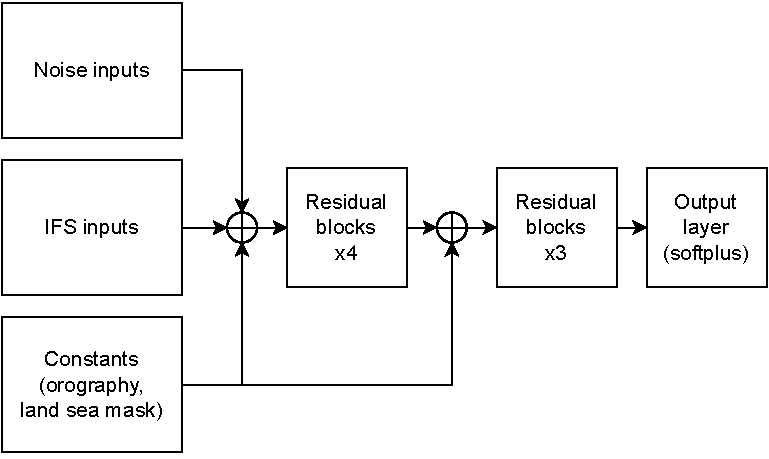
\includegraphics[width=\textwidth]{images/generator_2.drawio.pdf}
        \caption{}
        \centering
    \end{subfigure}
    \hfill
    \begin{subfigure}[c]{0.48\textwidth}
        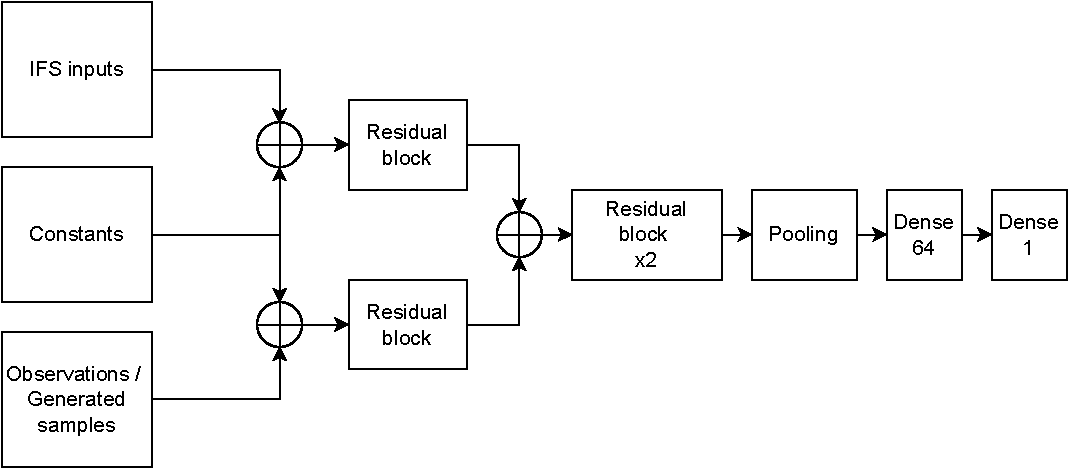
\includegraphics[width=\textwidth]{images/discriminator.drawio.pdf}
        \caption{}
        \centering
    \end{subfigure}
     \caption{The model architecture used in this work: a) the generator model and b) the discriminator model. For the generator, all inputs are first concatenated before being passed through 4 residual blocks. The output of this is concatenated with the constants again before being passed through another 3 residual blocks and a final output activation layer. The discriminator concatenates IFS inputs with constants, and constants with observations, which are then separately passed through residual block before being concatenated again, and passed through another 2 residual blocks. The outputs are then pooled and reshaped into a single number using two dense layers.}
    \label{fig:resnet}
\end{figure}    


In~\cite{harris_generative_2022} the training samples are chosen based on the total rainfall of each sample, such that wetter days are sampled more during training than drier days. However, the threshold used by Harris et. al.~for postprocessing UK rainfall was not appropriate for the drier region we are considering. We experimented with splitting data into rainfall by quartiles (according to mean rainfall over the image) and sampling the higher quartiles more often, but from visual inspection of the generated images this performed worse than just sampling uniformly over the training data, perhaps because we did not modify the loss function to compensate for the over-sampling.

Following standard practise for training neural networks, and based on the transformations applied in~\cite{harris_generative_2022}, we normalise the input variables: Precipitation input and variables are log normalised via $x \to \log_{10}(1 + x)$, whilst others were either divided by the maximum value, or normalised to fall within the maximum and minimum values (see Appendix~\ref{app:fcst_vars}).


Since our data volumes are relatively small compared to the amounts typically desired for deep learning, we used data augmentation to increase the variation of the samples the model sees, as this has been demonstrated to improve the generalisability of deep learning models~\citep{goodfellow_deep_2016}. To do so we randomly cropped the $270 \times 265$ images to smaller images of $200 \times 200$ during training. We also experimented with random rotations of multiples of $90^{\circ}$, however this led to a decrease in spatial realism (as measured by the quality of the RAPSD curve) and so was not used in the final run.



Similarly to the results in~\cite{harris_generative_2022}, we observed that the model quality during training (as measured by CRPS, RAPSD and visual inspection) was very variable, such that a validation set is required to pick the best model based on looking at summary statistics of CRPS, radially-averaged power spectral density, and ensemble mean-square error, plus visually assessing the realism of the samples. For this reason we kept out 4 months of validation data to be used to choose the best performing model (see Sec.~\ref{sec:data})

\subsection{Quantile mapping}
\label{subsec:qm}
Since it is known that raw IFS forecasts don't perform as well as post-processed forecasts in this region~\citep{vogel_skill_2018}, and IFS forecasts aren't intended to align with IMERG observations, we applied quantile mapping to the IFS forecasts (see e.g.~\cite{maraun_model_2017}) to provide a stronger baseline. Additionally, since our GAN predictions tended to over-predict at high rainfall values, we tested a variant of our model with quantile mapping applied to the output. In doing so we aimed to combine the strengths of both postprocessing methods to achieve an overall more accurate and realistic forecast. 
% A similar method to quantile mapping has been used within the African Monsoon Multidisciplinary Analysis 2050 (AMMA-2050) project, in which a model pipeline was built to produce reliable flood maps for future planning in Burkina Faso~\citep{senior_convection-permitting_2021}.


We used empirical quantile mapping rather than a distribution-based quantile mapping approach, since it has been demonstrated to work well~\citep{gudmundsson_quantile_2012}, and does not require a parametric distribution. Our method is based on the well-used methods outlined in~\cite{boe_statistical_2007, deque_frequency_2007, maraun_model_2017}, in which empirical cumulative density functions are calculated over the training period and used to create a mapping between the forecast quantiles and the observed quantiles. In general this means creating an estimate of the cumulative density functions $F_{f}$ and $F_{o}$ of the forecast and observations respectively, and mapping the forecast values $x_{f}$ to an adjusted value $\tilde{x}_f$ according to:
\begin{align}
    \tilde{x}_f = F^{-1}_o (F_f (x_f))
\end{align}

In~\cite{boe_statistical_2007}, percentiles at 1\% spacing are first calculated on the training set to find an approximation to the quantile distributions. Forecast values are then mapped into quantile values relative to the training data, and then converted into adjusted forecast values using the observed quantile values (using linear interpolation when the quantile falls between the known quantile values). 

Since the East African precipitation is low, there can be several quantiles that are 0; therefore if the forecast presents a 0 value there is no way to tell which quantile it belongs to. We follow the method in~\cite{boe_statistical_2007} and pick one of the 0-valued forecast quantiles at random, then assign the value of the matching observational quantiles. In practise, this can lead to low level noise on the corrected forecast, but replicates the high level statistics.

Based on the observation that evaluating the quantiles at high resolution was less important for lower quantiles, the step size between the quantiles was decreased towards the higher quantiles; so a step size of 0.01 was used up to 0.99, a step size of 0.001 used from 0.99 to 0.999, and so on until the step size cannot be reduced without having less than one data point per step (which leads to much higher resolution than seen in typical applications of quantile mapping), in order to capture the most extreme values. In practise this means going down to a minimum step size of $10^{-8}$, although note that each individual data point is far from independent and so the upper quantiles can be strongly affected by the presence of a single large weather system. This can lead to large errors due to the sampling variability in how the training and test sets are chosen, which we quantify using bootstrapping.


% In previous works, high rainfall values have been dealt with in different ways; for example in~\citep{leinonen_stochastic_2020} all assessments were made after converting the rainfall values to the [0,1] range. 

For data greater than the maximum value observed in training, we follow the additive uplift method~\citep{boe_statistical_2007, deque_frequency_2007} and add the uplift of the highest quantile for the IMERG and IFS data. For example, if $o_{\text{max}},f_{\text{max}}$ are the highest values seen in the training set for the observations and forecast respectively, then for any forecast value in the test data greater than $f_{\text{max}}$ we add the uplift $(o_{\text{max}} - f_{\text{max}})$ to it. 

\begin{figure}[h]

    \centering
    \hspace{-20mm}
    \begin{subcaptionblock}{.4\textwidth}
        \centering
        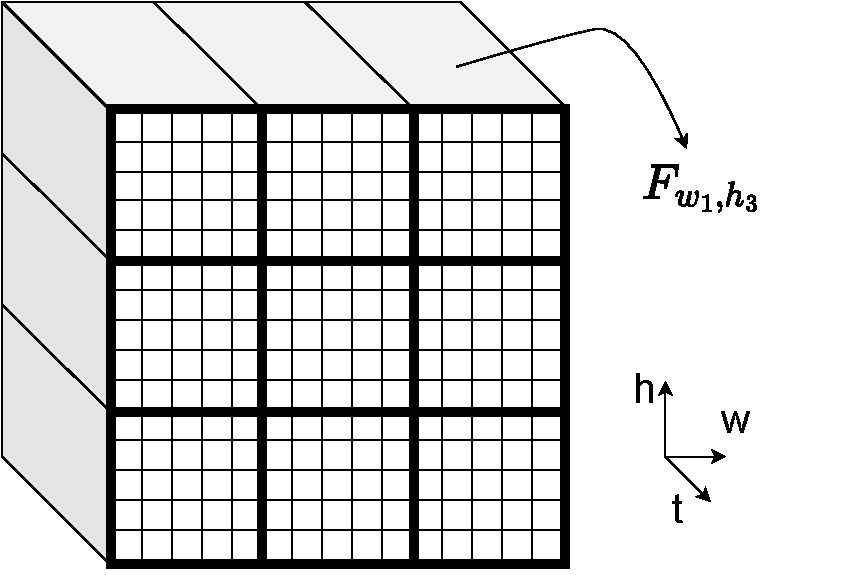
\includegraphics[width=\textwidth]{images/quantile_mapping.drawio.pdf}
        \caption{}\label{}
    \end{subcaptionblock}%
    \hspace{30mm}
    \begin{subcaptionblock}{0.20\textwidth}
        \centering
        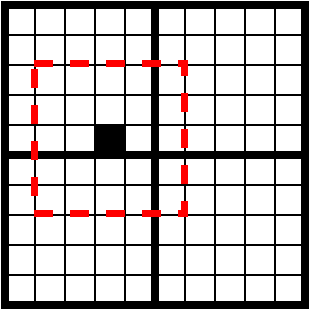
\includegraphics[width=\textwidth]{images/quantile_conv.drawio.pdf}
        \caption{}\label{}
    \end{subcaptionblock}%
    
        % \begin{subcaptionblock}{\label{cat}}
        % {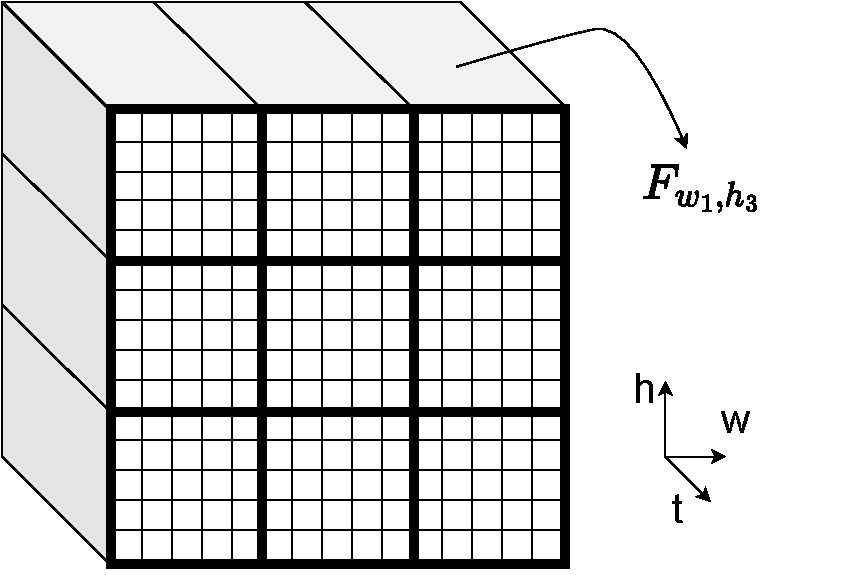
\includegraphics[width=0.5\textwidth]{images/quantile_mapping.drawio.pdf}}%
        % \subcaptionbox{\label{elephant}}
        % [0.5\textwidth]{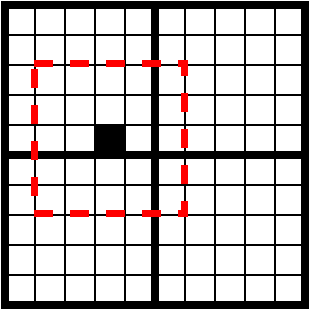
\includegraphics[width=0.25\textwidth]{images/quantile_conv.drawio.pdf}}
     % \begin{subfigure}[c]{0.48\textwidth}
     % \centering
     %     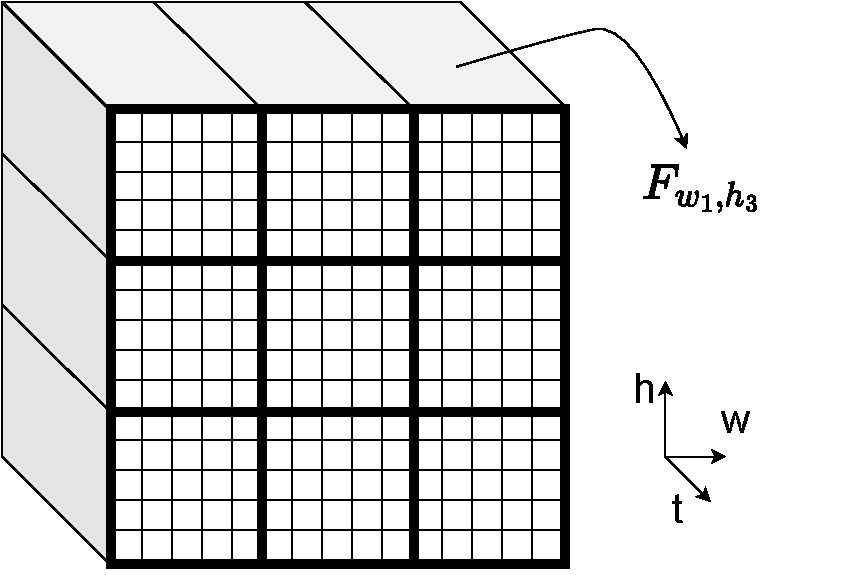
\includegraphics[width=\textwidth]{images/quantile_mapping.drawio.pdf}
     %     \caption{}
     %     \centering
     % \end{subfigure}
     % \hfill
     % \hspace{-10mm}
     % \begin{subfigure}[c]{0.25\textwidth}
     %     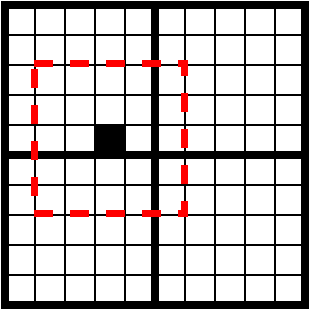
\includegraphics[width=\textwidth]{images/quantile_conv.drawio.pdf}
     %     \caption{}
     % \end{subfigure}
      \caption{a) Illustration of how grid cells are grouped together in order to estimate quantiles. In this example, the spatial domain is split into squares of $4 \times 4$ grid cells. Thus there are 9 separate square regions, and in each region the quantiles are calculated. b) to calculate a particular quantile for a grid point (in this case point (4,3)), we perform a weighted sum of the value of this quantile calculated in the square regions nearest to that pixel. The size of the weighting for each region is calculated by drawing a square around the grid cell (the red dashed line), and adding up how many small squares for each each region are contained in this square. In this example, the red dashed square covers 25 grid cells and the weightings would be $\frac{12}{25}$, $\frac{3}{25}$, $\frac{8}{25}$, $\frac{2}{25}$.}
     \label{fig:quantiles}
\end{figure}    


One further problem we encountered was the small number of independent training samples, which limited our ability to calculate accurate cumulative density. From experiments we found that the typical approach of quantile mapping the GAN at each grid point individually was not a robust approach for the extreme values. Therefore to calculate the quantiles we experimented with dividing the data into regions; spatially the region was grouped into equal sized squares (see Fig.~\ref{fig:quantiles} (a) for an illustration of this grouping). The intuition is that nearby points will have similar distributions and so we can gain accuracy by grouping nearby points together. 

To avoid any artefacts due to the edges of these domains, the quantiles for a given grid cell were calculated as a weighted average of the nearest squares; specifically, the quantiles used to update the values at grid cell $(m,n)$ are calculated as a weighted sum, where the weighting is calculated by drawing a square around $(m,n)$ and counting the number of grid points that fall into each quantile grouping (see Fig.~\ref{fig:quantiles} (b)). This is partly motivated by the ease of implementation, as this can be easily done by broadcasting the grouped quantiles to the same dimensions as the original grid, and using square convolutions with reflective padding to calculate the weighted versions of each quantiles. The length scale of the weighting window was chosen to be the same as the length scale of the quantile groupings, as this was empirically observed to produce reasonably smoothed values.

To evaluate the optimal grouping in the spatial domain, the mean square error of the quantiles after quantile mapping was evaluated over the whole domain. Using this method on the validation data, the cGAN performed best when quantiles were calculated uniformly over the whole domain, whilst the IFS forecast performed best when split into boxes of size $18 \times 18$. 





\section{Results}



\subsection{Climatological properties of the forecasts}
\label{sec:climatologic}
\begin{figure}[!ht]
     \centering
     \begin{subfigure}[h]{0.45\textwidth}
         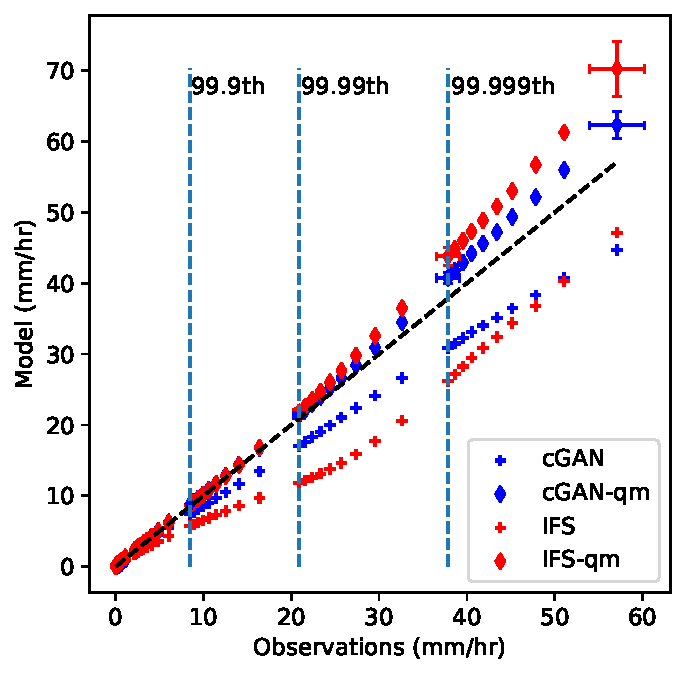
\includegraphics[width=\textwidth]{images/quantiles_total_final-nologs_217600.pdf}
         \caption{}
         \centering
     \end{subfigure}
     \hfill
     \begin{subfigure}[h]{0.5\textwidth}
         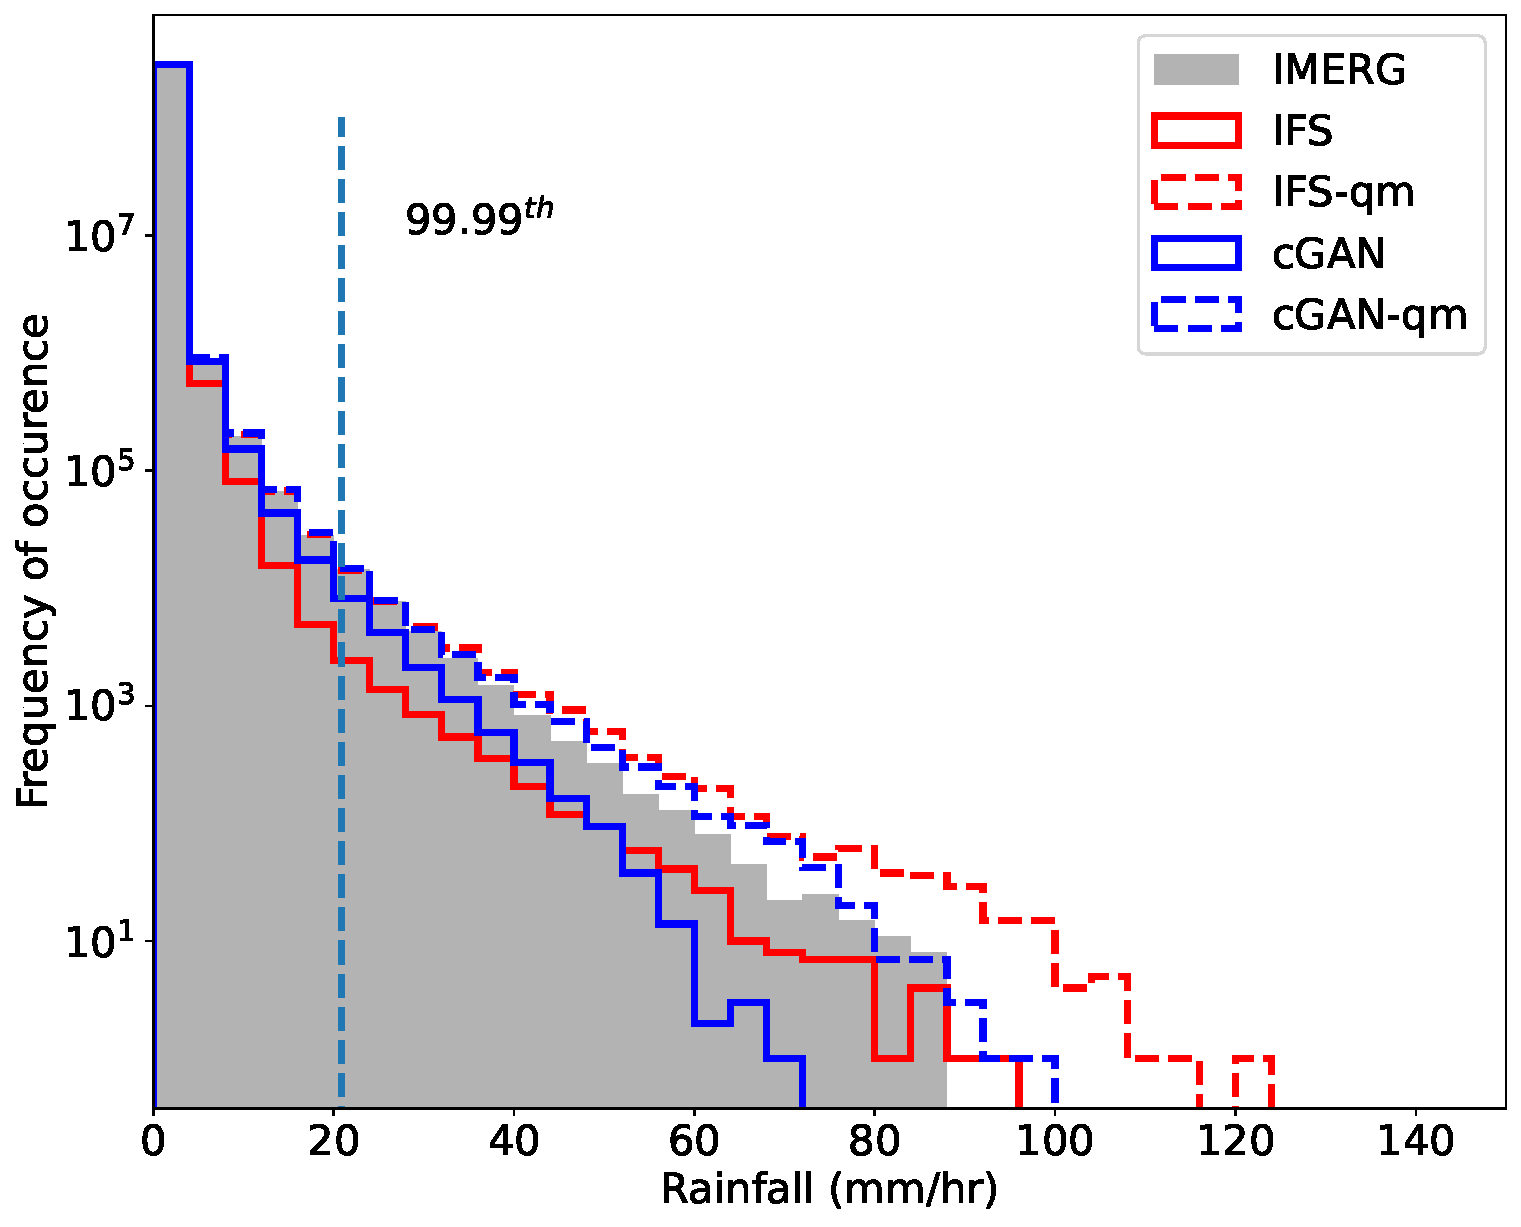
\includegraphics[width=\textwidth]{images/histograms_final-nologs_217600.pdf}
         \caption{}
        \centering
    \end{subfigure}
    \begin{subfigure}{0.48\textwidth}
     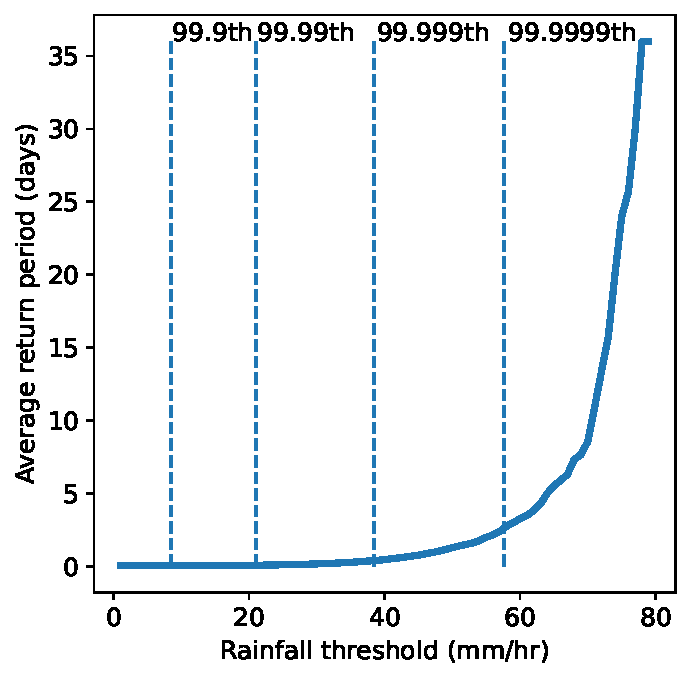
\includegraphics[width=\textwidth]{images/return_periods.pdf}
     \caption{}
     \end{subfigure}
     \centering
     \caption{a) Quantile-quantile plot, up to the $99.9999^{\text{th}}$ percentile. The black dashed line is the line along which a perfectly calibrated forecast would sit. The error bars indicate an estimate of 2 standard deviations from 1000 bootstrap samples b) A histogram showing the distribution of rainfall values; the vertical dashed blue line indicates the $99.99^{\text{th}}$ percentile of observed rainfall. The `qmap' suffix indicates that the forecast has been quantile mapped, as described in Sec.~\ref{subsec:qm}. c) The approximate return periods for different thresholds, calculated by finding the number of hours the threshold was exceeded for at least one pixel over the whole domain on the test set. The dashed lines indicating where the percentiles lie. }
     \label{fig:distribution}
\end{figure}

\begin{figure}[ht!]
     \centering
     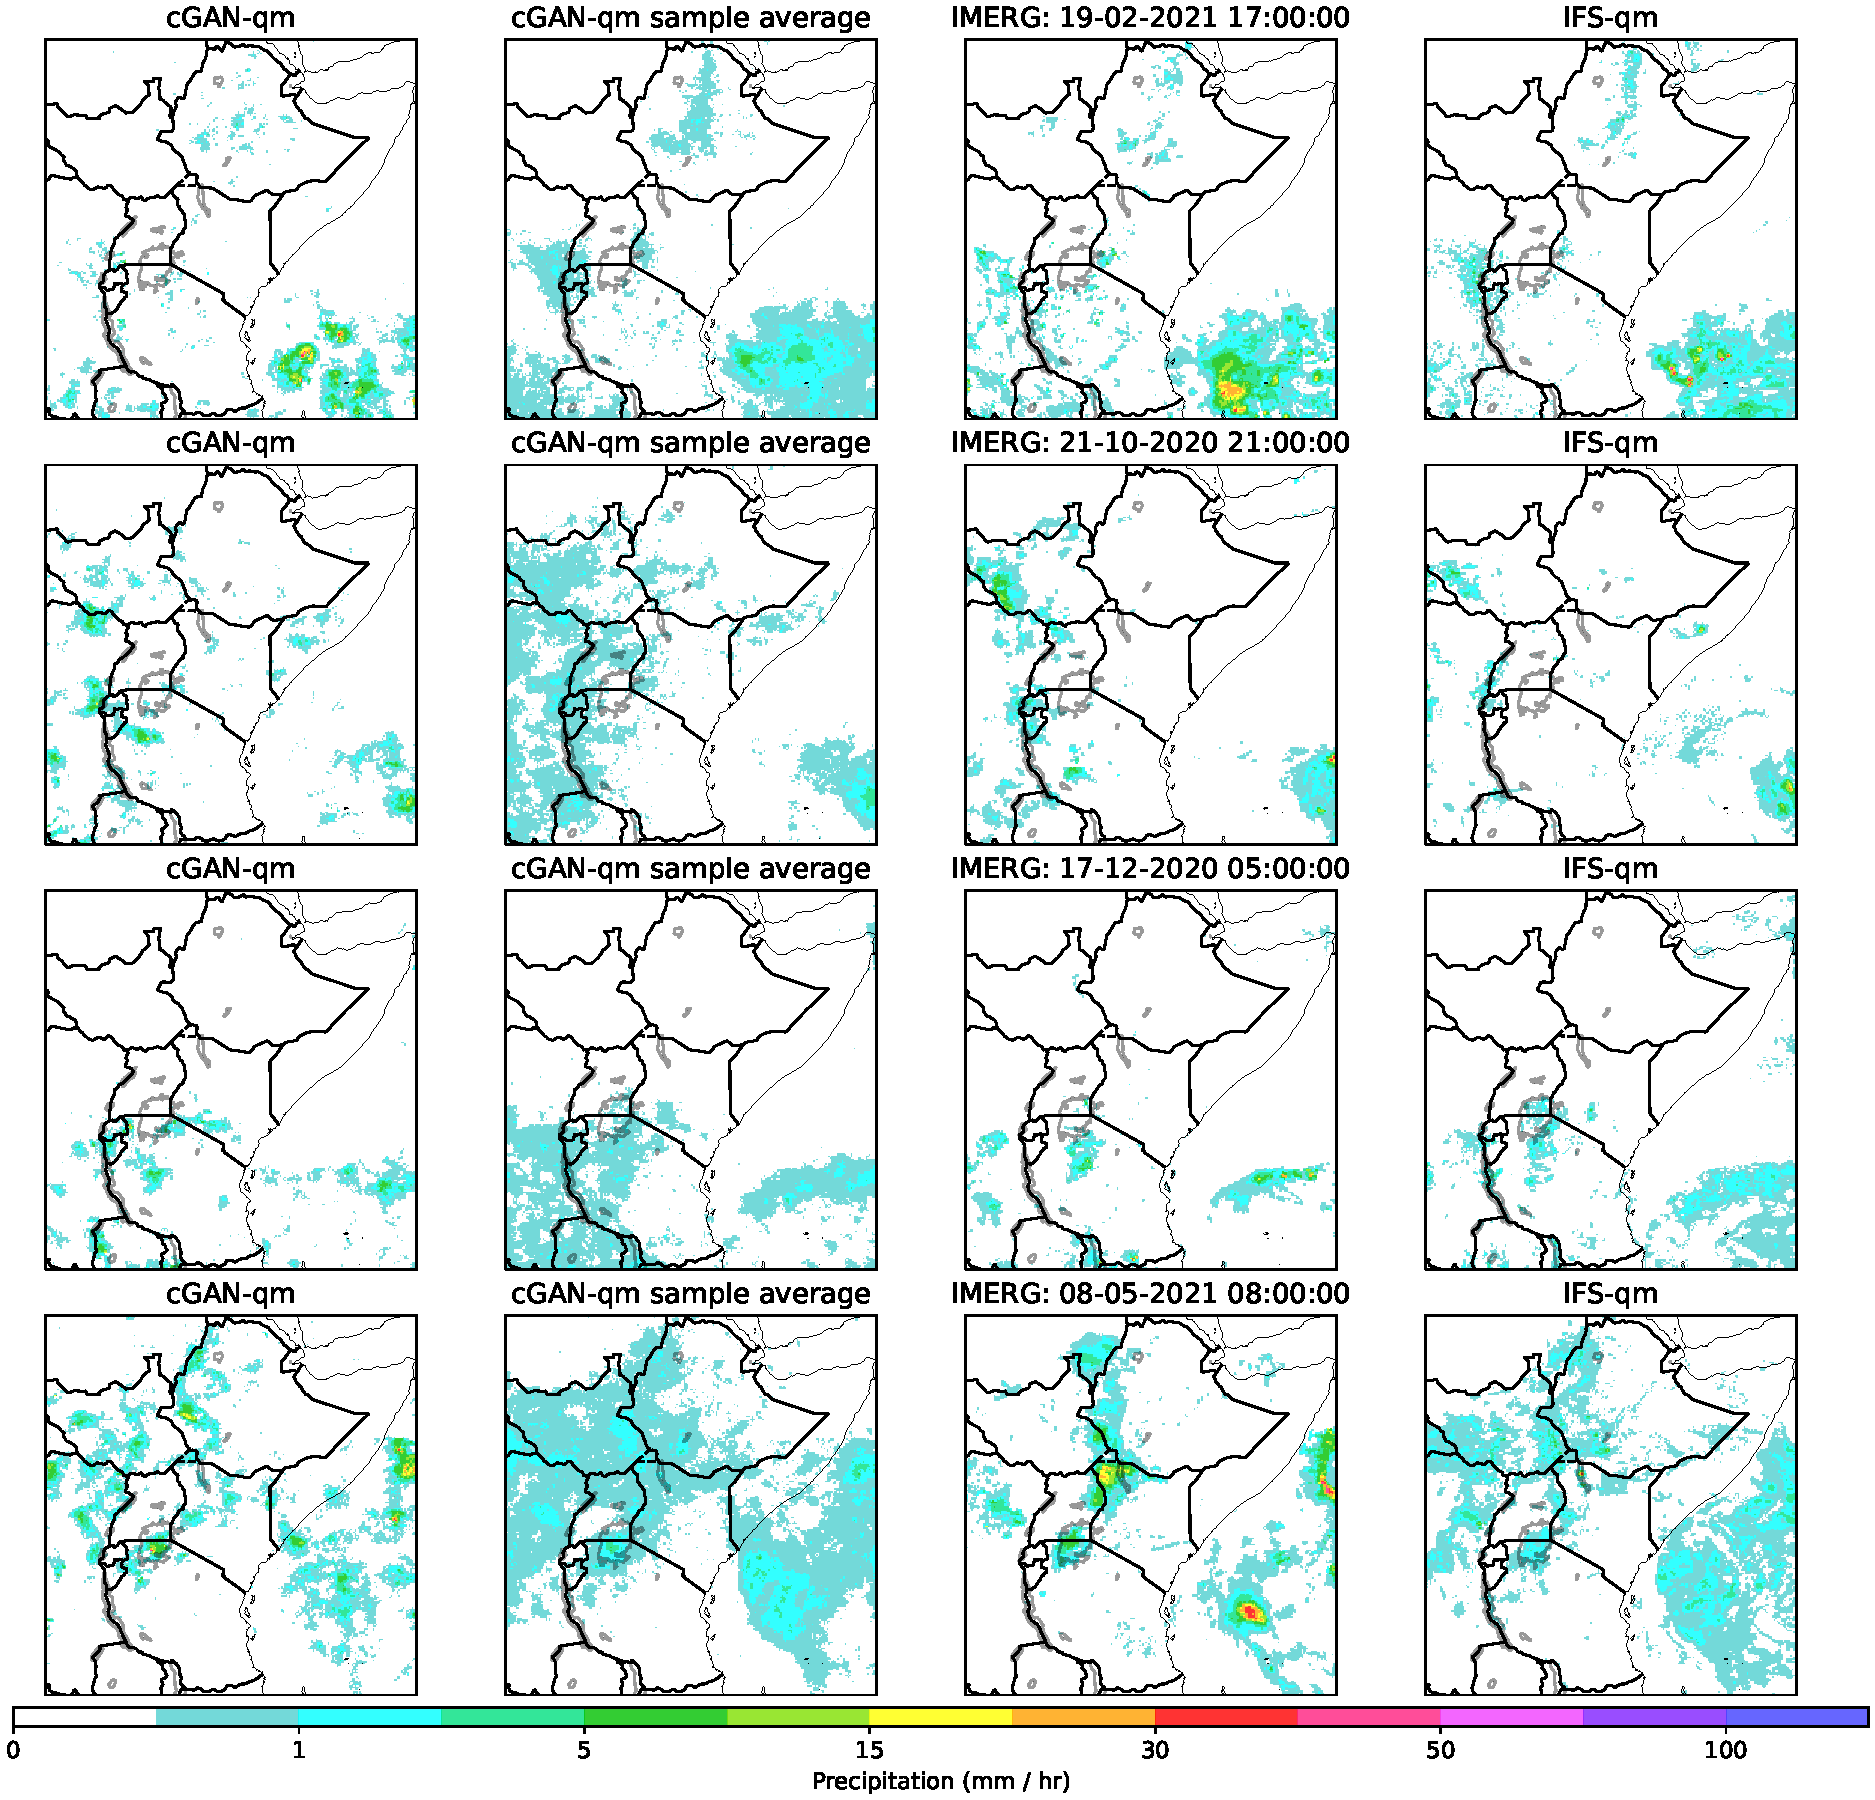
\includegraphics[width=1.05\textwidth]{images/cGAN_samples_IFS_final-nologs_217600.pdf}
     
     \caption{Example generated results from the cGAN-qm model, for a selection of hours throughout the test year, compared with IMERG observations and the IFS-qm model. Each row shows examples taken from the same timestamp. From left to right: a single member of the cGAN ensemble, the average of 20 cGAN-qm ensemble members, IMERG observations, the IFS forecast. }
     \label{fig:examples}
\end{figure}

\begin{figure}[!ht]
     \centering
     \begin{subfigure}{0.48\textwidth}
     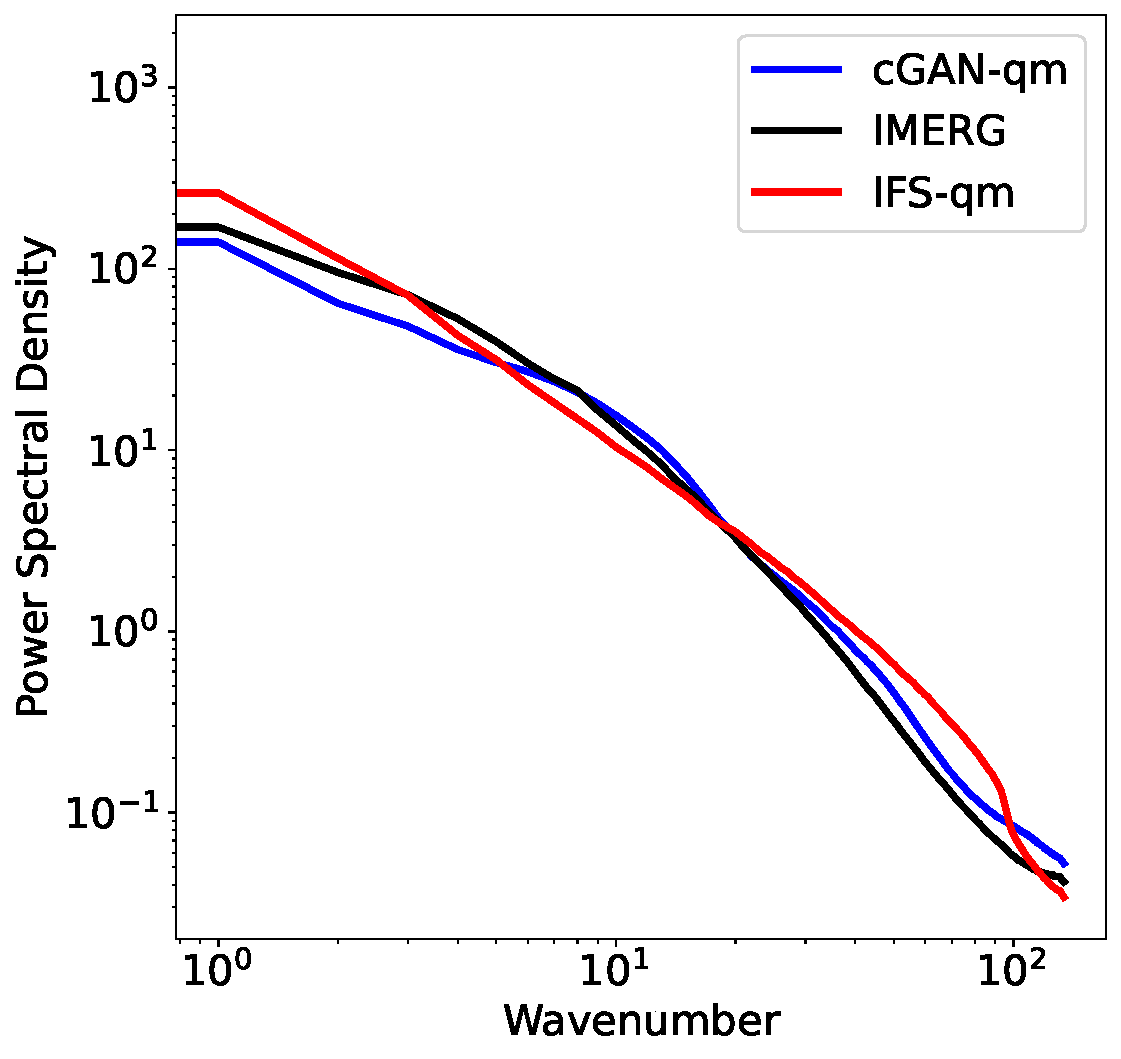
\includegraphics[width=\textwidth]{images/rapsd_final-nologs_217600.pdf}
     \caption{}
     \end{subfigure}
     
     \caption{a) Radially averaged power spectral density for the quantile mapped forecasts. 
}
     \label{fig:rapsd}
\end{figure}

\begin{figure}[!ht]
    \centering
    \begin{subfigure}{0.8\textwidth}
    \centering
     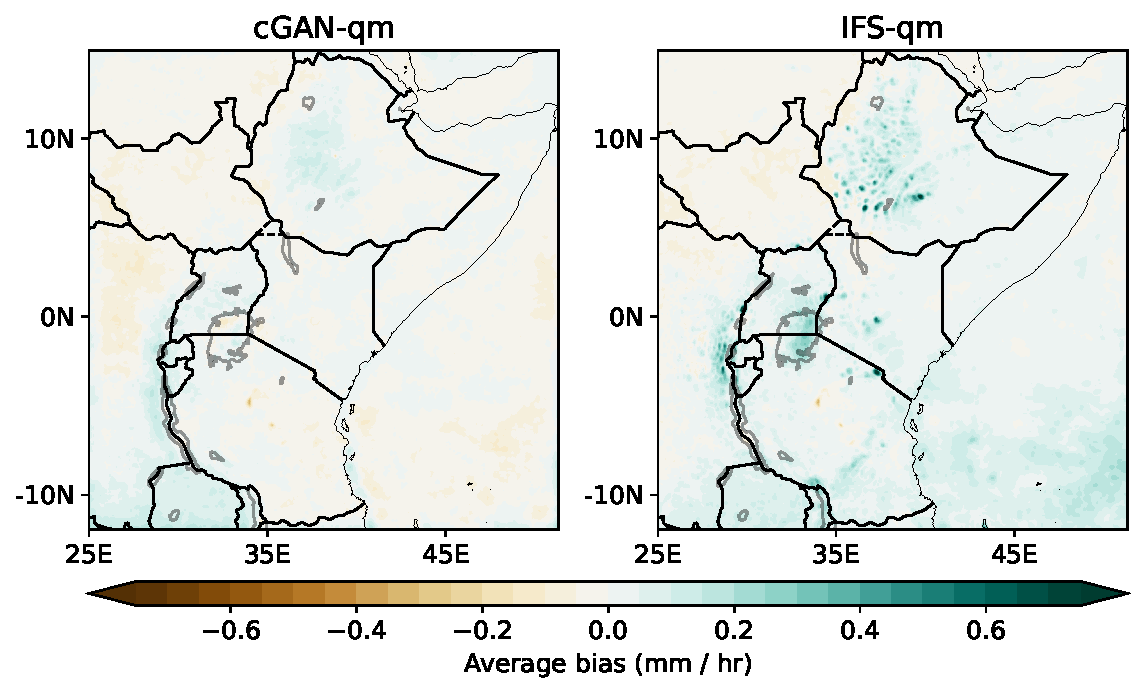
\includegraphics[width=\textwidth]{images/bias_final-nologs217600.pdf}
     \caption{}
     \end{subfigure}
     \begin{subfigure}{0.8\textwidth}
    \centering
     \includegraphics[width=\textwidth]{images/bias_std_final-nologs217600.pdf}
     \caption{}
     \end{subfigure}
    
     \caption{a) Average mean bias of the cGAN and IFS models b) Bias in the standard deviation for the cGAN-qm and IFS-qm models }
     \label{fig:bias}
\end{figure}

\begin{figure}
\centering
     \begin{subfigure}{\textwidth}
    \centering
     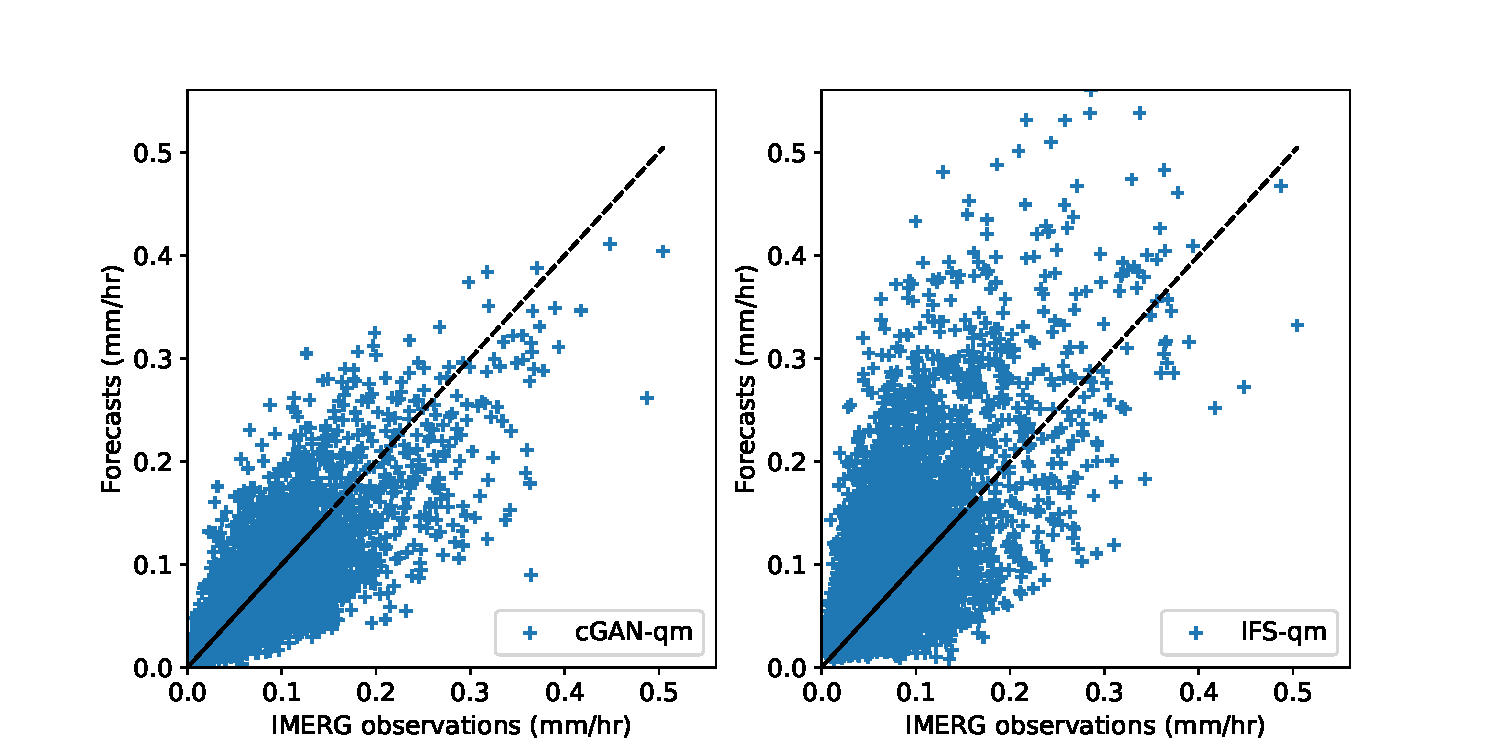
\includegraphics[width=\textwidth]{images/scatter_mean_final-nologs_217600.pdf}
     \caption{}
     \end{subfigure}
     \caption{Scatter plots of the domain averaged rainfall, for the IMERG observations against the cGAN-qm model (left) and IFS-qm model (right). In both plots the dashed black line represents the line that a perfect forecast would lie along. The Pearson correlation coefficient is 0.74 for the cGAN-qm model and 0.61 for the IFS data.}
     \label{fig:bias}
\end{figure}









\begin{figure}[t]
    \centering
     \begin{subfigure}[t]{0.33\textwidth}
 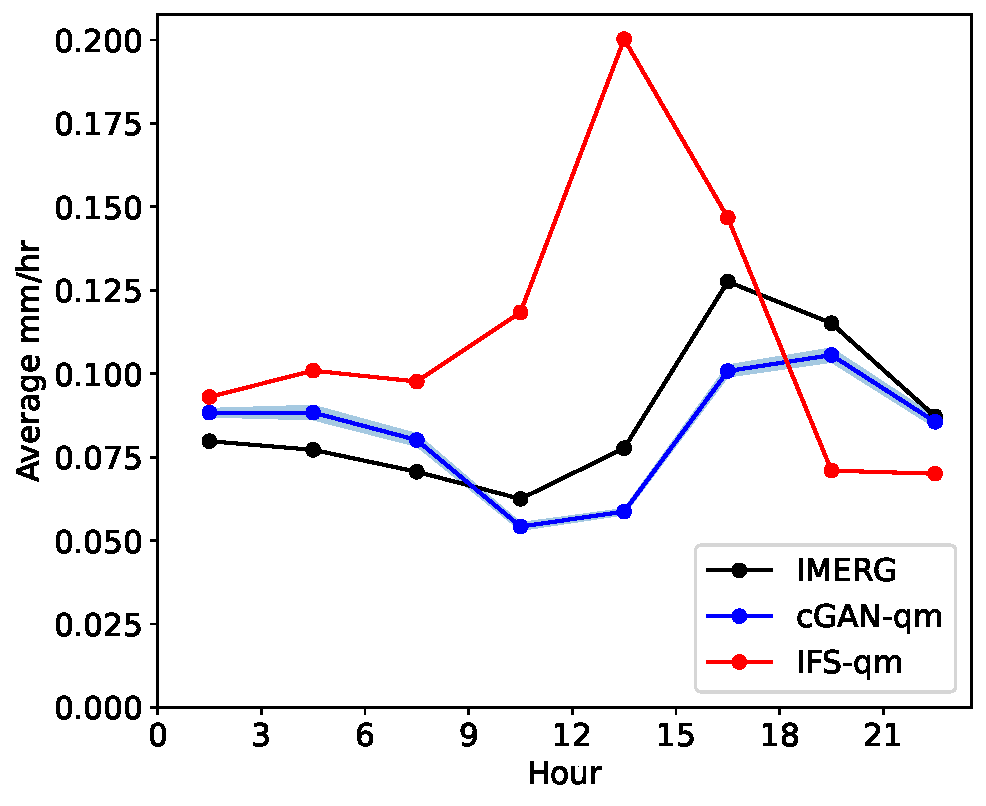
\includegraphics[width=\textwidth]{images/diurnal_cycle_mean_final-nologs_217600.pdf}
     \caption{}
     \end{subfigure}
     \begin{subfigure}[t]{0.32\textwidth}
     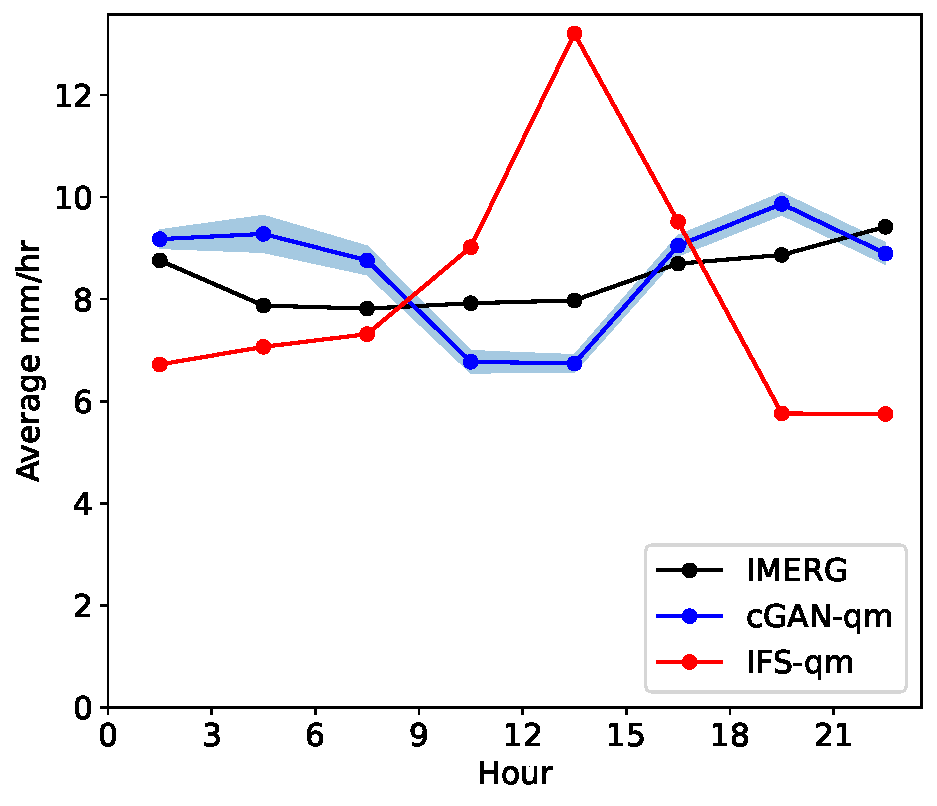
\includegraphics[width=\textwidth]{images/diurnal_cycle_quantile_999_final-nologs_217600.pdf}
     \caption{}
     \end{subfigure}
     \begin{subfigure}[t]{0.32\textwidth}
     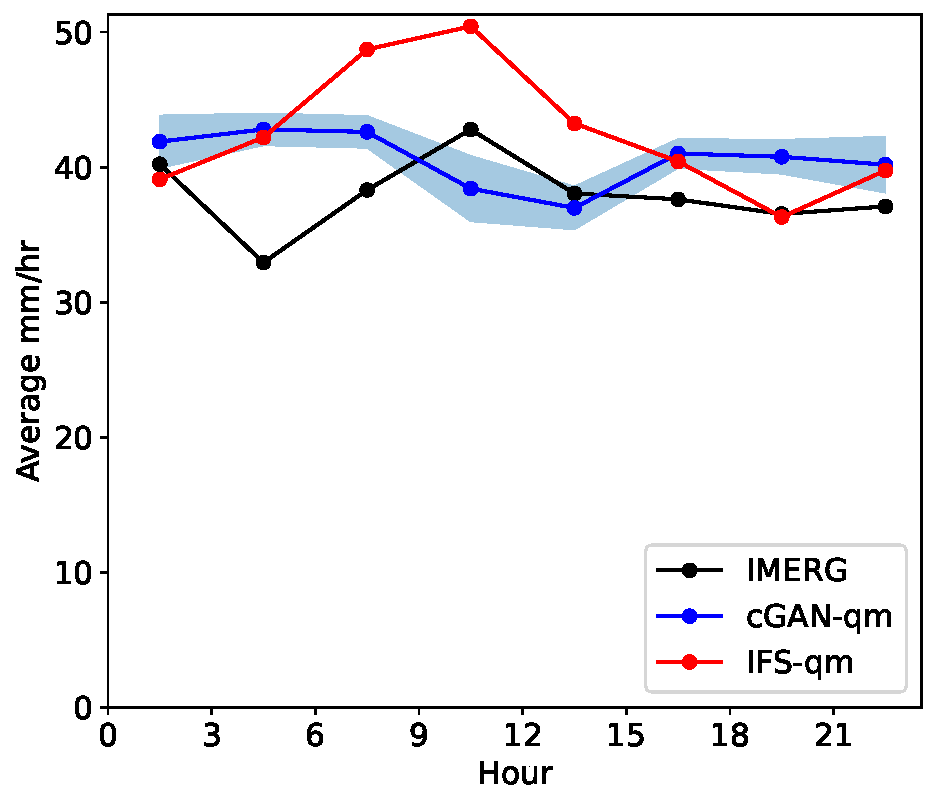
\includegraphics[width=\textwidth]{images/diurnal_cycle_quantile_99999_final-nologs_217600.pdf}
     \caption{}
     \end{subfigure}
     \caption{Evaluation of diurnal cycle in different summary statistics by hour (in local time) over the whole domain; a) mean rainfall, b) $99.9^{\text{th}}$ percentile, c) $99.999^{\text{th}}$ percentile. The shaded regions indicate $\pm2$ standard deviations about the mean. Note that rainfall at the $99.9^{\text{th}}$ percentile and above is mainly concentrated over Lake Victoria and over the sea.}
     \label{fig:diurnal}
\end{figure}

\begin{figure}[t]
\centering
\begin{subcaptionblock}{\textwidth}
        \centering
        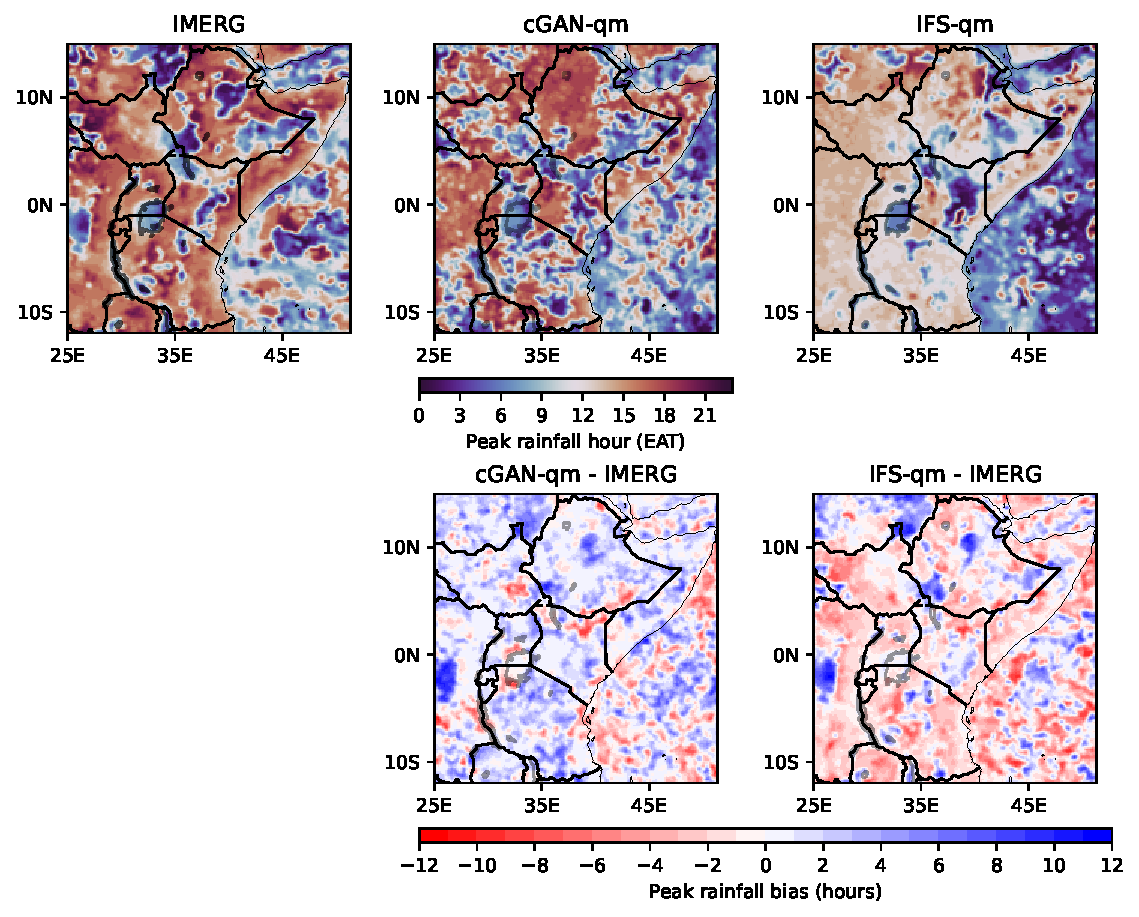
\includegraphics[width=\textwidth]{images/diurnal_cycle_map_All_final-nologs_217600.pdf}
        \caption{}\label{}
    \end{subcaptionblock}%
    \hfill
    % \begin{subcaptionblock}{\textwidth}
    %     \centering
    %     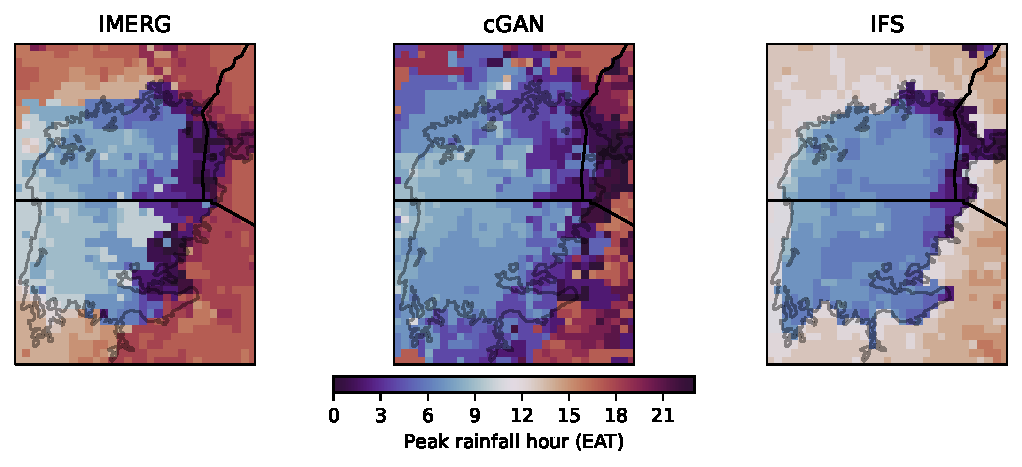
\includegraphics[width=\textwidth]{images/diurnal_cycle_map_Lake_Victoria_final-nologs_217600.pdf}
    %     \caption{}\label{}
    % \end{subcaptionblock}
     \caption{Map of peak rainfall hour averaged over the whole domain. A 3-hour moving average filter has been used to reduce noise in the time dimension before calculating the hour of peak rainfall.}
     \label{fig:peak_hour}
\end{figure}

 We first asses how well the forecasts capture the distribution of rainfall, by looking at a quantile-quantile plot and a histogram of rainfall distribution for 4000 samples taken from the test year, shown in Fig.~\ref{fig:distribution} (a) and (b) respectively. The raw model outputs are shown together with quantile-mapped outputs, indicated by a `-qm' suffix. From these we can see that the raw cGAN output is an improvement on the raw IFS output up to extremely high levels of rainfall (around 50mm/hr) beyond which point the IFS is closer to the distribution. Note that we wouldn't necessarily expect the GAN to align closely with the observed frequency distribution, since it is not explicitly trained to do so.

After both forecasts have been quantile mapped, they are much closer to the ideal line, with deviations at high quantiles which we attribute mainly to sampling variability. The scale of sampling variability was quantified by performing 1000 iterations of bootstrapping (see Sec.~\ref{sec:sample_var}) to estimate the standard deviation of the quantiles. These are shown in Fig.~\ref{fig:distribution}, where each error bar shows 2 standard deviations. It is likely that this is an underestimate of sampling variability, since there are correlations between samples that are unaccounted for, in which case it appears that the deviations of the quantiles from the diagonal is mainly due to sampling variability as expected. 


In order to also get a sense of how extreme these quantile values are, we plot the approximate return period in days for a range of thresholds in Fig.~\ref{fig:rapsd} (a), calculated over all hours in the test period. To calculate these, we find the total number of hours such that at least one point in the domain exceeds the threshold. Then the return period is estimated as the total number of hours in the test set, divided by the number of hours the threshold is exceeded. Finally this is divided by 24 to convert the answer to units of days. Note that due to correlations between hours, which artificially boost the number of times the threshold is exceeded, this will be a lower bound on the actual return period. Also note that the very high rainfall values (above around the $99.9^{\text{th}}$ percentile, $\sim20\text{mm/hr}$) are mainly concentrated over Lake Victoria and parts of the sea. 

Since these quantile mapped versions appear to much better forecasts, for the remaining diagnostics in this work we will focus on these quantile-mapped forecasts. Unless indicated otherwise, the following metrics are evaluated on a 4000 unique hours from the test period sampled uniformly over all dates from the test year.

We plot examples of the samples generated by the cGAN in Fig.~\ref{fig:examples}, for an ensemble size of 20. The generated samples appear to be fairly realistic, and the ensemble mean seems to correlate well with the locations and intensity of the observed rainfall. In the bottom row example (8am on 8th May 2021) we can see the cGAN removing some of the excess low rainfall seen over the land and see for the IFS-qm model. The top and bottom row examples also show both models not capturing the shape and maximum intensity of the high rainfall event occurring over the sea. To get a quantitative picture of how spatially realistic these rainfall patterns are, we plot the Radially Averaged Power Spectral Density (RAPSD) in Fig.~\ref{fig:rapsd}. From this we can that both quantile-mapped forecasts achieve similar results, with the cGAN slightly closer overall to the ideal line, and both forecasts showing opposite bias at the lowest wavenumbers, possibly due to sampling variability.

The plot of average bias in Fig.~\ref{fig:bias} (a) shows that on average the cGAN-qm under-predicts rainfall whilst the quantile-mapped IFS over-predicts. The cGAN also reduces the most prominent average biases of the IFS occurring over the Ethiopian highlands, Lake Victoria and the Western side of the East African rift, near Rwanda and Burundi. The effects on the bias in the standard deviation in Fig.~\ref{fig:bias} (b) are less obvious, there is some reduction in the sharpness of the peaks around the Ethiopian highlands, coastal regions and over the ocean, but there are also areas of increased negative bias in other parts of the ocean and in the western part of the domain over the Democratic Republic of Congo. The scatter plot in Fig.~\ref{fig:bias} shows how each model captures the domain-averaged rainfall; the cGAN-qm model is more tightly clustered around the ideal diagonal line, with the IFS-qm more spread out and tending to over-predict. This is reflected in the Pearson correlation coefficients; 0.74 for the cGAN-qm and 0.61 for the IFS-qm.



\begin{figure}[t]
    \centering
     \begin{subfigure}[t]{0.32\textwidth}
    \centering
 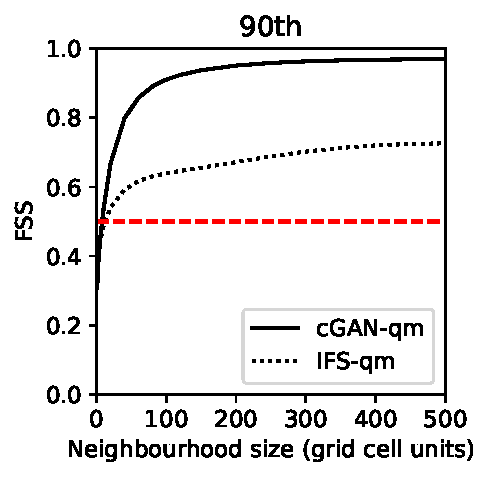
\includegraphics[width=\textwidth]{images/fss_q90th_final-nologs_217600.pdf}
     \caption{}
     \end{subfigure}
     \centering
     \begin{subfigure}[t]{0.32\textwidth}
     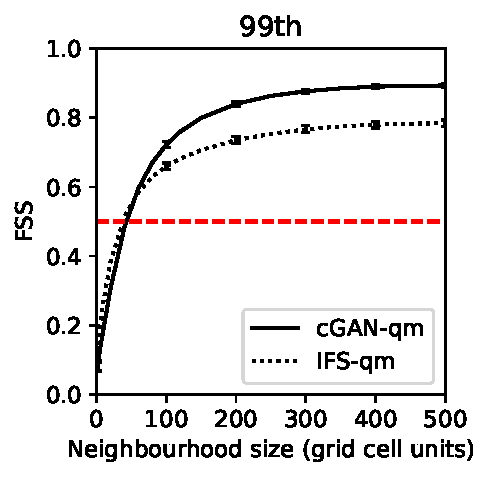
\includegraphics[width=\textwidth]{images/fss_q99th_final-nologs_217600.pdf}
     \caption{}
     \end{subfigure}
     \begin{subfigure}[t]{0.32\textwidth}
     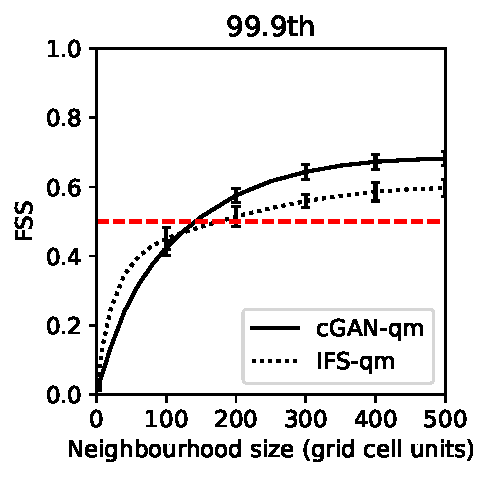
\includegraphics[width=\textwidth]{images/fss_q99.9th_final-nologs_217600.pdf}
     \caption{}
     \end{subfigure}
     \begin{subfigure}[t]{0.32\textwidth}
     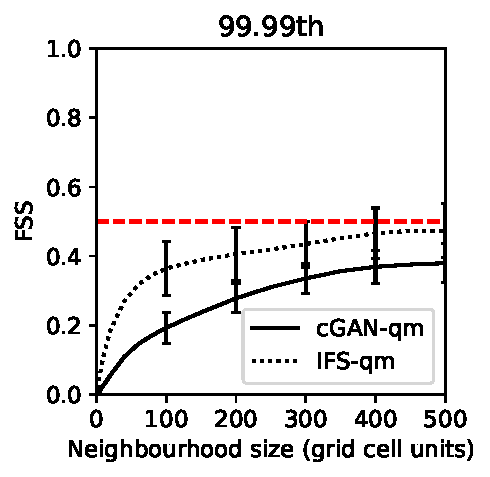
\includegraphics[width=\textwidth]{images/fss_q99.99th_final-nologs_217600.pdf}
     \caption{}
     \end{subfigure}
     \begin{subfigure}[t]{0.32\textwidth}
     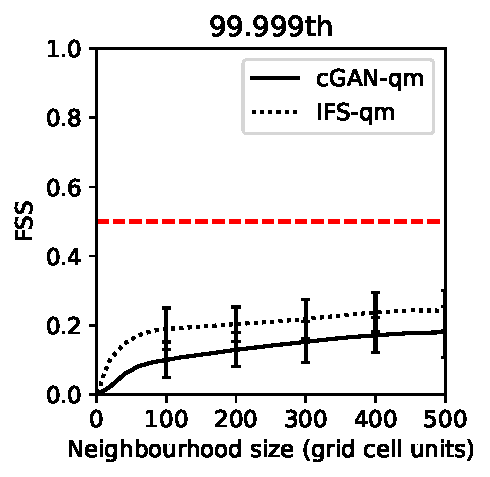
\includegraphics[width=\textwidth]{images/fss_q99.999th_final-nologs_217600.pdf}
     \caption{}
     \end{subfigure}
     \caption{Fractions Skill Score results for different quantile thresholds. The red dashed line indicates the `useful' criteria of 0.5 typically used to interpret this score. Error bars indicate $\pm2$ standard deviations estimated from bootstrapping with 50 samples. Note that rainfall at the $99.9^{\text{th}}$ percentile and above is mainly concentrated over Lake Victoria and over the sea. }
     \label{fig:fss}
\end{figure}

One source of error that the quantile mapping approach we use here is unable to adjust for is any bias in the diurnal cycle. Summary statistics of the rainfall as a function of hour are plotted in Fig.~\ref{fig:diurnal}, from which it is clear that the cGAN is making significant improvements to the diurnal cycle. The IFS forecast has a clear average bias around midday that is also prominent for high quantiles, whilst the cGAN is more aligned with observations.

We can gain insight into what regions are particularly driving this improvement from the plots of average peak rainfall hour in Fig.~\ref{fig:peak_hour}. The data is smoothed along the time axis using a centred moving average of length 3, in order to remove noise and make it easier to see any patterns in the data. The peak rainfall hour for the cGAN is fairly spatially noisy, but improvements can mainly be seen to occur on land. Note that the cGAN is not being given the hour as an input, but is instead using another variable as a proxy (e.g.~total incident solar radiation), which may explain the noisiness of the cGAN results. Looking at Lake Victoria, we can see that the cGAN correctly captures more of the nighttime maxima seen along the East coast of the lake and the morning maxima seen in the central and Western parts (see e.g.~\cite{woodhams_identifying_2019}), although it also tends to have a strong early bias in the land around the Western part of the lake.


\subsection{Event-based assessment}


We now look at how well each forecast is able to predict the occurrence of specific rainfall events, defined as the occurrence of rainfall above a certain threshold, starting with the Fractions Skill Score (FSS)~\citep{roberts_assessing_2008, roberts_scale-selective_2008}. In Fig.~\ref{fig:fss} we show plots of FSS for different quantile thresholds, where the quantiles are calculated over the whole domain rather than for each grid cell individually. Estimated error bars are also shown, based on bootstrapping with 50 resamples (which we expect to be a lower bound since the effects of correlation in time are not taken into account). 

The value that the FSS reaches at the maximum neighbourhood size indicates the bias in the frequency with which forecasts exceed the particular rainfall threshold, and so we can see that, up to thresholds around the $99.9^{\text{th}}$ percentile, the cGAN has lower overall bias. Above this threshold, whilst the IFS shows higher results on average, the effects of sampling variability are significant (especially given these error bars are an underestimate), and so it is unclear whether the IFS is genuinely performing better or has just performed better on a specific event in the data. 

The FSS is typically interpreted relative to the `useful' criteria of $\frac{1}{2} + \frac{f_O}{2}$, and we can see that, for thresholds up to around the $99.9^{\text{th}}$ percentile the cGAN crosses this line at slightly lower neighbourhood size. However, it is known that skilful forecasts can lie below this line~\citep{nachamkin_applying_2015, mittermaier_long-term_2013}, and we can see that the IFS achieves higher scores at lower neighbourhood sizes, which suggests improved skill at fine resolutions. 

Overall then, these results suggest that, for up to around the $99.9^{\text{th}}$ percentile the cGAN scores better. Above this level the sampling variability in the test set makes it hard to draw any robust conclusions, but for this test set the IFS shows better performance on average at the very high percentiles.



\begin{figure}[ht]
    \centering
     \begin{subfigure}[t]{0.45\textwidth}

     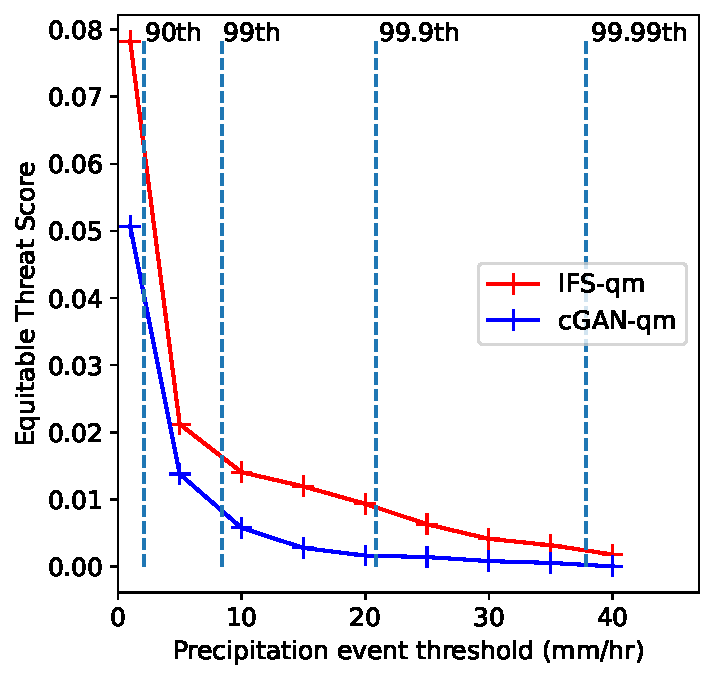
\includegraphics[width=\textwidth]{images/ets_final-nologs_217600.pdf}
     \caption{}
     \end{subfigure}
     \hfill
     \centering
     \begin{subfigure}[t]{0.49\textwidth}
     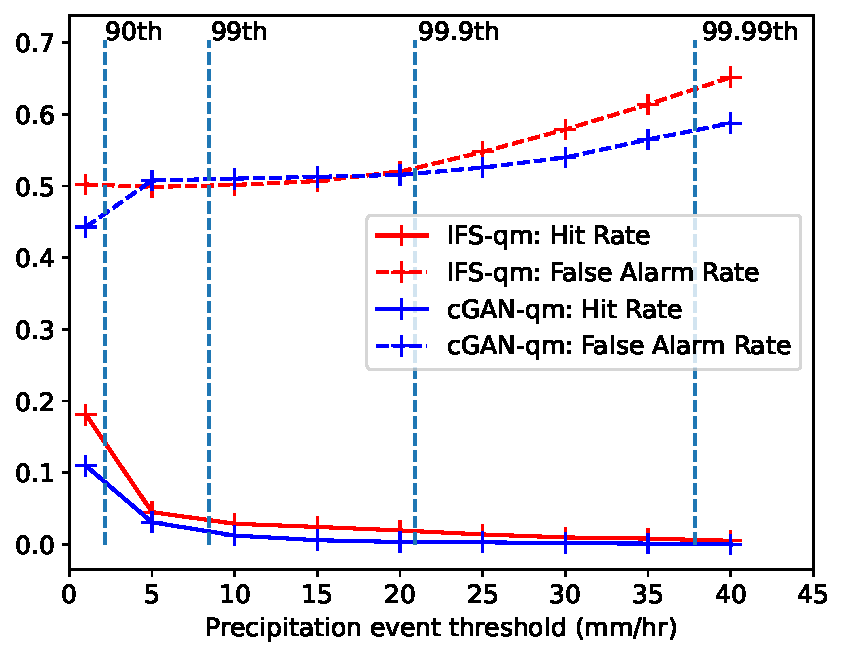
\includegraphics[width=\textwidth]{images/hit_rate_final-nologs_217600.pdf}
     \caption{}
     \end{subfigure}
     \caption{ a) Equitable threat score for the IFS-qm and cGAN-qm. b) Hit rate and False Alarm Rate for the IFS-qm and cGAN-qm models. Here an event is defined as whether not the rainfall at a particular grid cell exceed the rainfall threshold. Note that rainfall at the $99.9^{\text{th}}$ percentile and above is mainly concentrated over Lake Victoria and over the sea.}
     \label{fig:ets}
\end{figure}

We also asses the Equitable Threat Score (ETS)~\citep{schaefer_critical_1990, wilks_forecast_2019} at several thresholds over the whole domain, shown in Fig.~\ref{fig:ets} (a), at the single pixel level. This shows that the quantile mapped IFS tends to perform better by this metric, which is in agreement with the FSS results that show the IFS performing better at smaller length scales. It is also perhaps to be expected from the quantile-mapped IFS forecast having a heavier-tailed rainfall distribution, as demonstrated in Fig.~\ref{fig:distribution}. In Fig~\ref{fig:ets} (b) the Hit Rate (HR) and False Alarm Rate (FAR) are shown, from which we can see that performance at low rainfall values is predominantly driven by differences in HR, and for extremely high values the FAR tends to increase significantly.


        
\subsection{Assessment of ensemble calibration}


\begin{figure}[!ht]
    \centering
    \begin{subfigure}[t]{0.49\textwidth}
     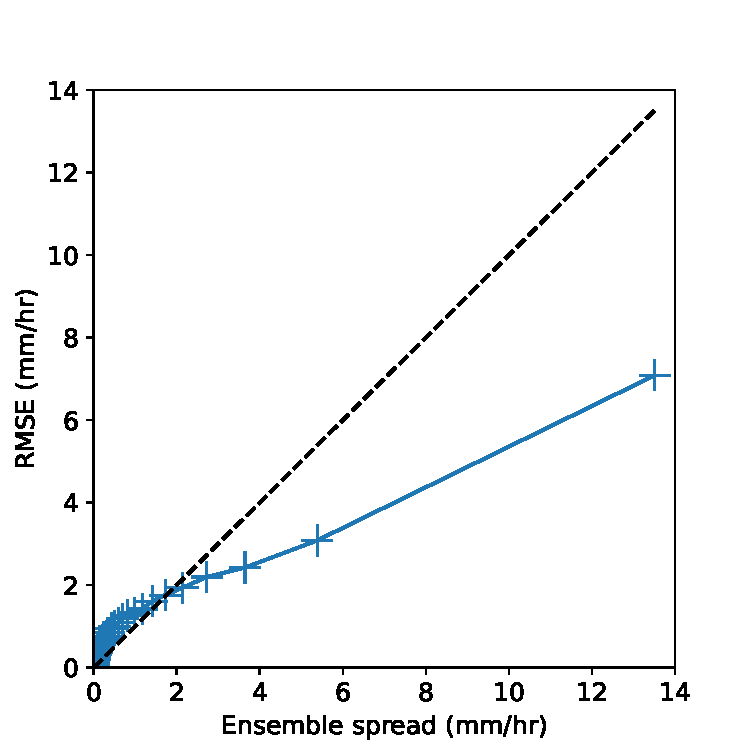
\includegraphics[width=\textwidth]{images/spread_error_final-nologs_217600.pdf}
     \caption{}
     \end{subfigure}
     \centering
    \begin{subfigure}[t]{0.49\textwidth}
     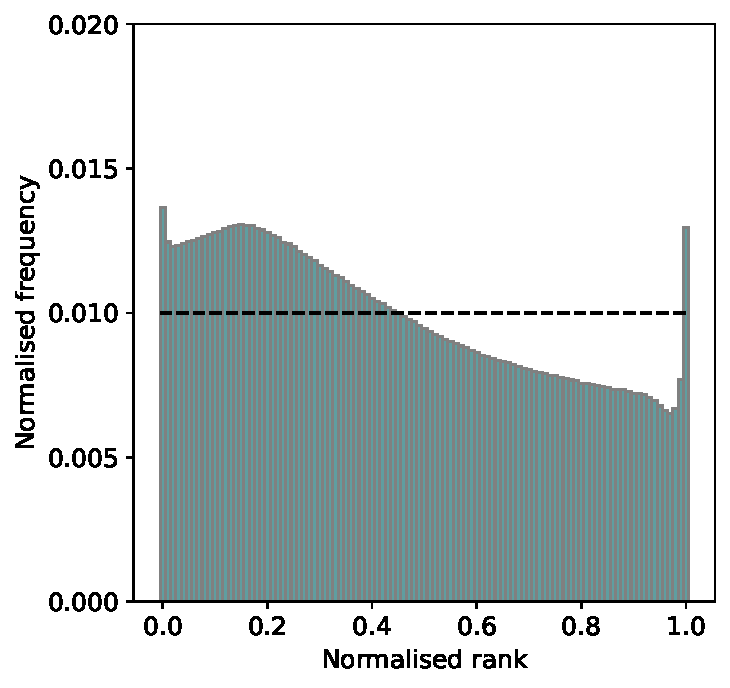
\includegraphics[width=\textwidth]{images/rank_hist_final-nologs_217600.pdf}
     \caption{}
     \end{subfigure}
     \centering
     \begin{subfigure}[t]{0.49\textwidth}
     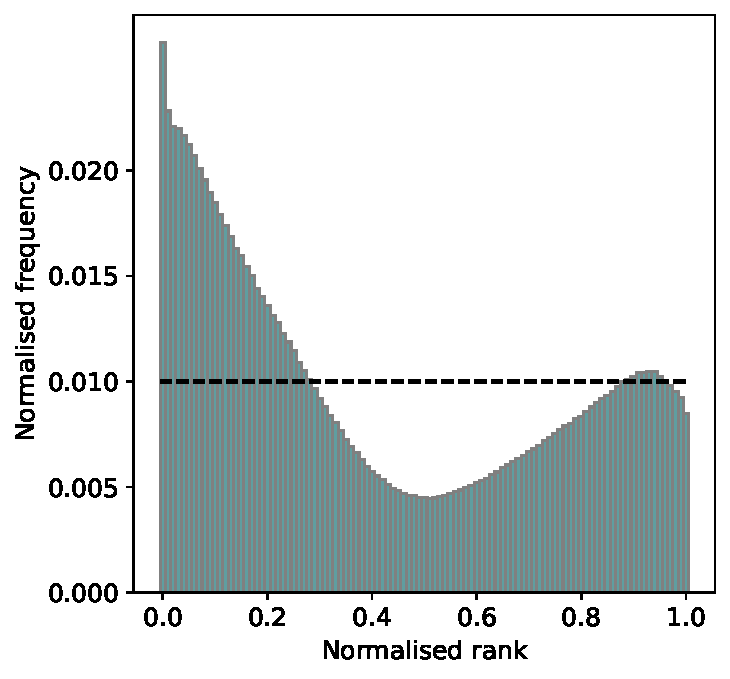
\includegraphics[width=\textwidth]{images/rank_hist_above_thr_final-nologs_217600.pdf}
     \caption{}
     \end{subfigure}
     \centering
      \begin{subfigure}[t]{0.49\textwidth}
     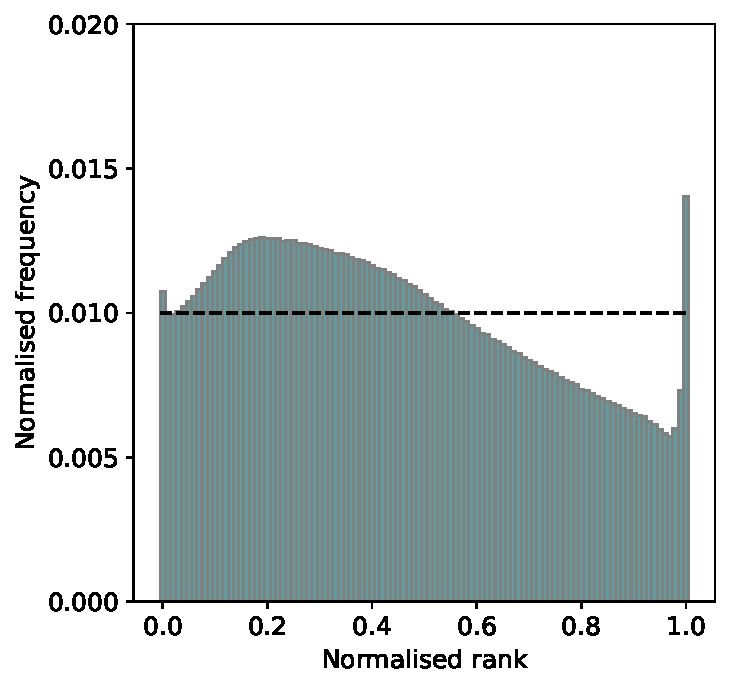
\includegraphics[width=\textwidth]{images/rank_hist_below_thr_final-nologs_217600.pdf}
     \caption{}
     \end{subfigure}
     
     
     \caption{Evaluation of the ensemble calibration of the cGAN, calculated using 500 samples of the cGAN with 100 ensemble members a) pixel-wise spread error, where the spread is split into 100 bins. b) pixel wise rank histogram, c) pixel wise rank histogram for pixels where the cGAN ensemble mean is $>0.1\text{mm/hr}$, c) pixel wise rank histogram for pixels where the cGAN ensemble mean is $\leq 0.1\text{mm/hr}$. For all plots, the dashed black line is the line that a perfectly calibrated ensemble would lie along. }
     \label{fig:ens_calib}
\end{figure}


We now focus on how well the cGAN ensemble is calibrated. Note that, since one of our aims is to be able to convert a deterministic forecast into an ensemble forecast, we do not have an ensemble forecast to compare with.

These results are assessed on 500 samples drawn uniformly over all days from the test year, each with 100 ensemble members. In Fig.~\ref{fig:ens_calib} (c) we show the spread error, where the spread is binned into 100 bins. From this we can see that the cGAN ensemble is slightly under-dispersive (i.e.~over-confident) for situations where there is low observed RMSE, but very over-dispersive (i.e.~under-confident) for situations where there is high RMSE. Since we would expect RMSE to roughly scale with the rainfall intensity, this suggests that the cGAN-qm model is over-confident at low rainfall values but under-confident at high rainfall values. Whilst the ensemble isn't calibrated perfectly, it is also reassuring to see that the cGAN has not fallen into the common failure mode of producing homogeneous images (which would produce extremely under-dispersive results).

The pixel-wise rank histogram in Fig.~\ref{fig:ens_calib} (b) also demonstrates that the ensemble deviates from the perfectly calibrated line, and appears to be made up of a mixture of behaviours. In general it is hard to uniquely attribute forecast behaviour from a rank histogram~\citep{hamill_interpretation_2001}; a U-shaped distribution can be indicative of under-dispersion of the ensemble, but can also be a mixture of over- and under-forecasting biases. 

In order to shed light on this, we also calculate rank histograms conditioned on the value in the cGAN-qm ensemble mean. In Fig.~\ref{fig:ens_calib} (c) and (d) we show rank histograms conditioned on the cGAN ensemble mean being $>0.1\text{mm/hr}$ and $\leq 0.1\text{mm/hr}$, respectively. In Fig.~\ref{fig:ens_calib} (c) we can see a clear U-shape for the high values, indicating under-dispersion, and a tendency to predict higher than the observations. From Fig.~\ref{fig:ens_calib} (d) we can see that the dominant behaviour at low rainfall intensity is over-prediction and over-dispersion. 

There is also an apparent contradiction between the spread-error plot result and the rank histogram: The spread-error plot appears to show decreasing dispersion with high rainfall values, while the rank histogram appears to show under-dispersion at high rainfall values. An explanation for this could be down to the fact that the rank histogram measures ordering and is insensitive to the particular error values, unlike the spread-error. Then potentially the spread-error is being skewed by a small number of forecasts that produce very high predictions, which doesn't show up on the rank histograms.

Another explanation for this contradiction is that, rather than being a U-shape indicating under-dispersion, the rank histogram in Fig.~\ref{fig:ens_calib} (c) is a mixture of systematic under- and over-forecasting, such that on average the cGAN over-forecasts, which also leads to large spreads.

    
% \section{Evaluation on extreme test set}

% ...


% A visual inspection of samples produced by the cGAN (Fig.~\ref{fig:cgan_sample}) confirms that it produces realistic spatial rainfall patterns; general features seem to be that the cGAN removes some of the wet bias at low intensities, and more accurately represent the high intensity rainfall. We use the radially-averaged spectral density as a measure of the spatial structure of the forecasts, shown in Fig.~\ref{fig:metrics}(a); this shows that the cGAN samples have a closer resemblance to the spectral density than the original forecast (although the cGAN tends to overpredict at high wavenumber - corresponding to smaller length scales). Compared to the quantile mapped forecast, the cGAN appears to do better at medium-range wavenumbers, but less well at higher wavenumbers. The cGAN also successfully corrects the position of the peak in diurnal cycle of the IFS (shown for the whole region in Fig.~\ref{fig:metrics}(c)), although it shows an overprediction in the peak height.

% Quantile-quantile plots reveal that the cGAN is able to correct the forecast bias up to the 99.99th percentile. However, beyond this there is extreme overprediction of high rainfall; this is an effect noted in~\citep{harris_generative_2022}, for which they introduced a rainfall threshold to cut off extremely high values. Also all the scores in~\citep{leinonen_stochastic_2020} were calculated after converting the rainfall to the range [0,1], and so any errors in intensity would not have registered in their analysis. A natural question to ask is why the discriminator in the GAN is unable to pick up on these extreme intensities; one explanation could be that GAN discriminators are known to be poor at learning for any frequency components in the image that have low magnitude (which in this case are the high frequency components)~\citep{schwarz_frequency_2021}. 

% note that the results capture the earlier peak rainfall in southeastern Lake Victoria, as mentioned in \citep{finney_implications_2019}.


\section{ Conclusions}


In this work we have investigated how a particular implementation of a conditional Generative Adversarial Network can improve the ECMWF IFS HRES forecast over equatorial East Africa, and how well it can create an ensemble based on this deterministic forecast. Quantile mapping was applied to the IFS forecast (IFS-qm) to provide a strong baseline, and also to the cGAN output (cGAN-qm) in order to leverage the strengths of both quantile mapping and machine learning.


The cGAN-qm and IFS-qm rainfall distributions are comparable, with both models tending to over-predict at high rainfall values (more than around 20mm/hr), although it is likely that much of this high quantile behaviour is due to sampling variability and the particular properties of the training and testing years. The cGAN-qm removes some of the biases in the IFS-qm model, as demonstrated by plots of the average bias and a scatter plot of domain averaged rainfall.

The most substantial improvement effect seen was for the diurnal cycle, which is known to be particularly problematic for conventional NWP models such as the IFS HRES to capture. The cGAN-qm model demonstrated a substantial improvement in the average diurnal cycle over the whole domain, which persisted when looking at the diurnal cycle of high quantiles. A map of peak rainfall intensity further demonstrated this, although there is still a significant amount of spatial noise in the cGAN peak rainfall hour, perhaps because time is not passed explicitly and the model has not yet learnt the full relationship between the variables and the diurnal cycle (and perhaps not all of the relevant variables are provided to enable it to do so).

To assess the ability of the model to predict events at a range of scales, the Fractions Skill Score (FSS) was used. Up to a high percentile ($99.9^{\text{th}}$) the cGAN-qm shows generally higher FSS scores, particularly at larger neighbourhood sizes, demonstrating that the cGAN-qm has lower bias in the frequency of pixels exceeding the threshold. For extremely high rainfall values, the IFS-qm forecast had a higher score although when sampling variability is taken into account this difference is not significant. To evaluate the ability of each forecast to predict rainfall events at individual points and times, without accounting for spatial structure, the Equitable Threat Score (ETS) was used; the IFS-qm model achieved higher ETS at all thresholds, although neither forecast demonstrated high enough scores to be considered usable.



The calibration of the cGAN ensemble was assessed via a spread-error plot and rank histograms. Both diagnostics indicate under-dispersion at high rainfall values and over-dispersion at lower rainfall values. This separation was partly identified through rank histograms conditioned on the ensemble mean being above or below a small threshold (01mm/hr).

Overall, these results highlights the subtlety in identifying the improvements a cGAN can bring; whilst the cGAN can significantly improve the raw IFS forecast, a strong baseline is crucial to find the areas where the cGAN can outperform conventional postprocessing methods. Compared to the quantile mapping baseline the improvements are mainly in the diurnal cycle and the scores for rainfall events at low to medium rainfall intensities. 


One limitation is the lack of a baseline ensemble to compare probabilistic forecasts against; towards the end of this project, the ECMWF IFS released ensemble forecast data at the same resolution, so going forward it would be ideal to compare our ensemble predictions to these. 
 
In general, forecast postprocessing and verification is more meaningful when done towards a particular forecast user's needs, as this allows informed decisions to be made as to how to improve the model. So in future work it would be best to target a particular use-case for these forecasts, and this would also inform the best way to train the generative model. Since the focus of this work is on short term forecasting to aid with early warnings for flooding, it would be particularly insightful to use the output of the cGAN model as input to a hydrology model, and assess any potential benefits there may be. Over Lake Victoria, one of the main hazards is high winds, and whilst rainfall can serve as a proxy for when these winds may happen, it would be interesting to see how the cGAN would perform at forecasting wind speeds as well. The performance of these models on unseen extreme rainfall was also not evaluated; however we have held back a part of the data (the 2018 long rains) for a future evaluation.

We have mostly considered the entire domain as a whole, but as the domain behaviour is very heterogeneous, it could be better to train and/or evaluate the models over more smaller areas of more meaningful significance, such as river basins prone to flooding, areas managed by a particular disaster relief agency, areas grouped by climatological similarity, or areas where impacts are particularly high (e.g.~high population density areas). 

Our quantile mapping baseline is also limited in that it cannot modify the diurnal cycle, and 

There are many possible standard machine learning methods that would be good to try, such as spectral normalisation or batch normalisation after the convolutions as used in~\cite{ravuri_skilful_2021}, or a more nuanced scheme to weight the rainier days more heavily, which given the particularly dry climate seen here may well make significant improvements if performed properly. There are also additional terms we could use in the loss function, such as RAPSD, pooled spatial values, or Fractions Skill Score, that we may expect to help produce well-calibrated forecasts.

There may also be additional variables that are not currently fed into the model that could be useful. For example, location-specific parameters such as latitude or longitude, topography, or an embedding of location as done in~\cite{rasp_neural_2018}. There is potential that these would improve the results by learning behaviours that are specific to a region and that only weakly depend on the input variables we have. Also we implicitly assume that the IFS forecast captures all of the useful information about phenomena such as the Indian Ocean Dipole, Madden-Julian oscillations and ENSO, which are known to be important factors for forecasting extreme rainfall~\citep{wainwright_extreme_2021, palmer_drivers_2023}. It would be insightful to use indexes of these drivers as additional input, and/or sea surface temperatures in relevant parts of the Indian Ocean. It would be interesting as well to include the initial state of the forecast, if available, to see whether the machine learning model is able to correct for errors in how the IFS evolves this initial state.


In \cite{thiery_early_2017} they demonstrate the usefulness of land storm activity from the previous afternoon in predicting morning storm activity over Lake Victoria, so this would be useful additional information to have if it is available to a forecast system. Given the significant effect of Lake Victoria on the local climate, a separate lake and sea mask may also be effective in improving forecasts in that area, and it may be better to train a separate model over that region.

There are also other promising machine learning models that would be interesting to compare with, to see if performance improvements can be made. Particularly promising approaches would be diffusion models~\citep{addison_machine_2022}, since they appear to perform well and are easier to train, and models trained directly on a suitable loss function such as the energy score.

\bibliography{references_z}

\appendix

\section{Forecast variables used}\label{app:fcst_vars}
The IFS variables used to train the model are shown in Table~\ref{tab:vars}, definitions taken from~\citep{ecmwf_parameter_2023}.

The preprocessing methods mentioned in the table are as follows, using the year 2017 as the reference period:
\begin{itemize}
    \item Minmax: calculate the minimum $d_{\text{min}}$ and maximum $d_{\text{max}}$ over the reference period, and then transform each value $v$ according to $(v - d_{\text{min}}) / (d_{\text{max}} - d_{\text{min}})$.
    \item Max: calculate the and maximum $d_{\text{max}}$ over the reference period, and then transform each value $v$ according to $v  / d_{\text{max}}$.
    \item Log: Transform each value $v$ according to $\log_{10}(1+v)$.
\end{itemize}
\begin{table}[ht!]
\centering
\begin{tabular}{c | c | c } 
 \hline
 Variable name & Symbol & Pre-processing applied \\ [0.5ex] 
 \hline\hline
 2 metre temperature &2t & Minmax  \\
 Convective available potential energy &cape & Log \\
 Convective inhibition &cin & Max \\
Convective precipitation &cp & Log \\
Surface pressure & sp & Minmax  \\
Total column cloud liquid water &tclw & Max \\
Total column vertically-integrated water vapour&tcwv & Log \\
Top of atmosphere incident solar radiation&tisr & Max \\
Total precipitation &tp & Log \\
Relative humidity at 200hPa  &r200 & Max \\
Relative humidity at 700hPa  &r700 & Max \\
Relative humidity at 950hPa  &r950 & Max \\
Temperature at 200hPa &t200 & Minmax \\
Temperature at 700hPa  &t700 & Minmax \\
Eastward component of wind at 200hPa &u200 & Max \\
Eastward component of wind at 700hPa &u700 & Max \\
Northward component of wind at 200hPa&v200 & Max \\
Northward component of wind at 700hPa &v700 & Max \\
Vertical velocity at 200hPa &w200 & Max \\
Vertical velocity at 500hPa &w500 & Max \\
Vertical velocity at 700hPa &w700 & Max \\
 \hline
\end{tabular}

\caption{IFS variables used to train the model, as well as the normalisation applied to each variable. See text for description of the different preprocessing types.}
\label{tab:vars}
\end{table}


\end{document}
